\documentclass[12pt,letterpaper]{article}

% =========================================================
% PAQUETES
% =========================================================
\usepackage[utf8]{inputenc}
\usepackage[T1]{fontenc}
\usepackage[spanish,es-tabla]{babel}
\usepackage{geometry}
\usepackage{setspace}
\usepackage{amsmath}
\usepackage{amssymb}
\usepackage{graphicx}
\usepackage{float}
\usepackage{booktabs}
\usepackage{array}
\usepackage{hyperref}
\usepackage{xcolor}
\usepackage{listings}
\usepackage{caption}

% =========================================================
% CONFIGURACIÓN DE PÁGINA
% =========================================================
\geometry{
    left=2.5cm,
    right=2.5cm,
    top=2.5cm,
    bottom=2.5cm
}

\onehalfspacing

\hypersetup{
    colorlinks=true,
    linkcolor=black,
    citecolor=black,
    urlcolor=blue
}

% =========================================================
% CONFIGURACIÓN DE CÓDIGO
% =========================================================
\lstdefinestyle{irafstyle}{
    basicstyle=\ttfamily\small,
    backgroundcolor=\color{gray!8},
    frame=single,
    breaklines=true,
    columns=fullflexible,
    keepspaces=true
}

\lstset{style=irafstyle}

% =========================================================
% COMANDO PARA FIGURAS PENDIENTES
% =========================================================
\newcommand{\figplaceholder}[2]{
\begin{figure}[H]
    \centering
    \fbox{
        \parbox[c][6cm][c]{0.85\textwidth}{
            \centering
            \textbf{Agregar figura aquí}\\[0.3cm]
            \texttt{#1}\\[0.2cm]
            #2
        }
    }
    \caption{#2}
\end{figure}
}

% =========================================================
% TÍTULO
% =========================================================
\title{
    \textbf{Reducción de imágenes CCD y fotometría instrumental usando IRAF}\\
    \large Análisis de imágenes de M92 y M41 mediante herramientas de IRAF
}

\author{
    Santiago Serrano Perico\\
    Departamento de Física\\
    Universidad de los Andes
}

\date{\today}

\begin{document}

% =========================================================
% PORTADA
% =========================================================
\begin{titlepage}
    \centering
    
    \vspace*{2cm}
    
    {\Large \textbf{Reducción de imágenes CCD y fotometría instrumental usando IRAF}\par}
    
    \vspace{1cm}
    
    {\large Análisis de imágenes de M92 y M41 mediante herramientas de IRAF\par}
    
    \vspace{2cm}
    
    \textbf{Autor:}\\
    Santiago Serrano Perico
    
    \vspace{1cm}
    
    \textbf{Asesor:}\\
    Jose Alejandro Garcia Varela
    
    \vspace{1cm}
    
    \textbf{Departamento de Física}\\
    Universidad de los Andes
    
    \vfill
    
    \today
    
\end{titlepage}

\tableofcontents
\newpage

% =========================================================
\section{Resumen}
% =========================================================

El presente informe resume tres talleres desarrollados con el software IRAF para el análisis de imágenes astronómicas CCD. El trabajo se organizó en tres etapas principales: la reducción CCD de imágenes del cúmulo globular M92, la identificación manual de estrellas mediante herramientas interactivas de visualización y la realización de fotometría de apertura sobre imágenes de M92 y M41.

En el primer taller se realizó la reducción preliminar de las imágenes \texttt{m92010}, \texttt{m92011}, \texttt{m92014} y \texttt{m92015}, aplicando procedimientos como inspección de encabezados, corrección por overscan, recorte, bias y flat field. En el segundo taller se trabajó con la visualización de imágenes y la identificación manual de estrellas usando \texttt{display} e \texttt{imexamine}. En el tercer taller se realizó fotometría de apertura, primero sobre una imagen de M92, especialmente \texttt{m92011}, y posteriormente sobre el archivo multiextensión \texttt{M41.fits}, separando sus canales \texttt{blue}, \texttt{red} y \texttt{green}.

El análisis permitió estudiar la importancia de parámetros como el FWHM, el sigma del fondo de cielo, el radio de apertura y el umbral de detección. Además, se generaron archivos de coordenadas, archivos de magnitudes instrumentales y gráficas de magnitud instrumental contra error fotométrico, con el fin de evaluar la calidad de las mediciones obtenidas.

% =========================================================
\section{Introducción}
% =========================================================

La astronomía observacional moderna utiliza detectores CCD, \textit{Charge-Coupled Devices}, para registrar imágenes digitales del cielo. Un CCD está formado por una matriz de píxeles sensibles a la luz. Durante una exposición, los fotones incidentes generan electrones dentro del detector y la carga acumulada en cada píxel se convierte posteriormente en una señal digital. Por esta razón, una imagen CCD no es únicamente una representación visual del cielo, sino una matriz numérica que contiene información cuantitativa sobre la luz recibida por cada píxel.

De acuerdo con Howell \cite{howell2006}, los CCD son detectores fundamentales en astronomía debido a su alta eficiencia cuántica, bajo ruido de lectura y capacidad para producir mediciones reproducibles. Estas propiedades permiten realizar imágenes científicas, astrometría, espectroscopía y fotometría. En este trabajo, el interés principal es la fotometría, es decir, la medición del brillo de estrellas a partir de imágenes digitales.

\subsection{IRAF como herramienta de análisis astronómico}

IRAF, \textit{Image Reduction and Analysis Facility}, es un entorno de trabajo diseñado para la reducción y análisis de datos astronómicos. Fue ampliamente utilizado en astronomía profesional para procesar imágenes CCD, espectros y otros tipos de datos observacionales. IRAF funciona mediante una línea de comandos en la cual el usuario ejecuta tareas organizadas en paquetes. Cada paquete agrupa herramientas relacionadas con una etapa específica del análisis.

Por ejemplo, el paquete \texttt{images} contiene tareas generales para manipulación de imágenes, el paquete \texttt{ccdred} contiene tareas para reducción de datos CCD, y los paquetes \texttt{digiphot} y \texttt{apphot} contienen herramientas para fotometría de apertura. En este proyecto se usaron tareas como \texttt{imhead}, \texttt{display}, \texttt{ccdproc}, \texttt{imexamine}, \texttt{qphot}, \texttt{daofind}, \texttt{tvmark}, \texttt{phot} y \texttt{txdump}.

Una característica importante de IRAF es que muchas tareas tienen archivos de parámetros. Estos parámetros controlan cómo se ejecuta cada tarea. Algunos parámetros son solicitados directamente al usuario cuando se ejecuta el comando, mientras que otros son parámetros ocultos que pueden modificarse mediante \texttt{epar}. Esto permite ajustar el comportamiento de cada tarea según el tipo de imagen, el detector, el filtro, el tamaño de las estrellas y el objetivo del análisis.

En este trabajo IRAF se utilizó junto con DS9, un visor de imágenes astronómicas. IRAF envía las imágenes a DS9 mediante la tarea \texttt{display}, y desde allí es posible inspeccionar visualmente el campo, cambiar contraste y brillo, identificar estrellas, revisar detecciones y verificar resultados de fotometría.

\subsection{Señales presentes en una imagen CCD}

Una imagen CCD cruda no contiene solamente la luz proveniente del objeto astronómico. También incluye diferentes contribuciones instrumentales asociadas al detector y al proceso de lectura. Por esta razón, antes de realizar mediciones científicas es necesario aplicar un proceso de reducción. El objetivo de la reducción CCD es remover o corregir estas señales adicionales para que las cuentas medidas representen de forma más confiable la luz proveniente del cielo.

De manera simplificada, el valor registrado en un píxel de una imagen cruda puede entenderse como:

\begin{equation}
    I_{\text{cruda}} = I_{\text{objeto}} + I_{\text{cielo}} + I_{\text{bias}} + I_{\text{dark}} + \text{efectos de sensibilidad del detector}.
\end{equation}

Por tanto, para obtener una imagen útil para fotometría es necesario corregir el nivel electrónico del detector, eliminar regiones no científicas, corregir variaciones de sensibilidad y, cuando sea necesario, considerar la corriente oscura.

\subsection{Bias}

El \textit{bias} es una señal electrónica añadida por el sistema de lectura del CCD incluso cuando no llega luz al detector. Esta señal aparece porque el detector necesita un nivel base distinto de cero para poder leer correctamente los valores de los píxeles. Por eso, aun en una exposición de tiempo cero o muy corto con el obturador cerrado, la imagen no tiene valores nulos, sino un nivel electrónico de fondo.

Las imágenes bias se toman con tiempo de exposición cero y con el detector cerrado. Su propósito es medir ese nivel electrónico base. Normalmente se combinan varias imágenes bias para construir un \textit{master bias}, que luego se resta de las imágenes científicas y de calibración. Esta corrección es importante porque, si no se elimina el bias, las cuentas medidas en las estrellas estarían artificialmente aumentadas por una señal que no corresponde a luz astronómica.

\subsection{Overscan}

El \textit{overscan} es una región del CCD que se lee junto con la imagen, pero que no corresponde a una zona iluminada del detector. Es decir, son columnas o filas adicionales que no contienen señal astronómica. Estas regiones permiten estimar el nivel electrónico de lectura en cada imagen individual.

La ventaja del overscan es que permite corregir variaciones del nivel de bias que pueden cambiar de una imagen a otra. Mientras que el master bias representa una corrección promedio, el overscan permite medir el nivel electrónico presente en una exposición específica. En IRAF, la corrección por overscan se puede aplicar dentro de \texttt{ccdproc}, especificando la región de overscan mediante parámetros como \texttt{biassec}.

\subsection{Trim o recorte}

El \textit{trim} consiste en recortar la imagen para conservar solamente la región útil del detector. Después de aplicar la corrección por overscan, las columnas o filas correspondientes al overscan ya no son necesarias para el análisis científico. Además, algunas imágenes pueden contener bordes, regiones defectuosas o zonas no iluminadas que deben eliminarse.

El recorte permite trabajar únicamente con la zona científica de la imagen. En IRAF, esta región se define mediante el parámetro \texttt{trimsec}. Por ejemplo, una región de recorte puede tener la forma:

\begin{lstlisting}
trimsec = [1:315,2:510]
\end{lstlisting}

Esto indica qué columnas y filas se conservan después del recorte. La selección correcta de la región de trim es importante porque afecta todas las etapas posteriores, incluyendo alineación, detección de estrellas y fotometría.

\subsection{Dark current}

La corriente oscura, o \textit{dark current}, es una señal producida por electrones generados térmicamente dentro del detector, incluso cuando no hay luz incidente. Esta señal depende de la temperatura del CCD y del tiempo de exposición. En detectores bien refrigerados y con exposiciones no muy largas, puede ser pequeña, pero en otros casos debe corregirse.

Las imágenes dark se toman con el obturador cerrado y con el mismo tiempo de exposición que las imágenes científicas. Al combinar varias imágenes dark se puede construir un \textit{master dark}, que luego se resta de las imágenes. En este proyecto, la corrección por dark depende de las características de los datos disponibles y de si la contribución térmica es significativa frente al resto de fuentes de ruido.

\subsection{Flat field}

El \textit{flat field} corrige variaciones de sensibilidad entre píxeles y variaciones en la iluminación del campo. En una imagen CCD, no todos los píxeles responden exactamente igual ante la misma cantidad de luz. Además, el sistema óptico puede producir viñeteo, motas de polvo o gradientes de iluminación. Estas variaciones afectan directamente las cuentas medidas en las estrellas.

Para corregir este efecto se toman imágenes de una fuente aproximadamente uniforme, llamadas flats. Estas pueden ser flats de cielo, flats de domo o flats obtenidos con una pantalla iluminada. Los flats se corrigen primero por bias y luego se normalizan. La imagen científica se divide por el flat normalizado, de modo que las diferencias de sensibilidad se compensen.

La corrección de flat field es especialmente importante en fotometría, porque una estrella ubicada en una zona menos sensible del detector podría parecer artificialmente más débil si no se aplica esta corrección.

\subsection{Reducción CCD}

La reducción CCD combina las correcciones anteriores para transformar una imagen cruda en una imagen lista para análisis científico. En términos generales, el proceso puede resumirse como:

\begin{equation}
    I_{\text{reducida}} =
    \frac{
    I_{\text{cruda}} - I_{\text{bias}} - I_{\text{dark}}
    }{
    I_{\text{flat normalizado}}
    }.
\end{equation}

En la práctica, el proceso exacto depende de los datos disponibles. Para las imágenes de M92 trabajadas en este informe, la reducción se realizó con IRAF usando tareas del paquete \texttt{ccdred}, especialmente \texttt{ccdproc}. Esta tarea permite aplicar corrección por overscan, recorte, bias y flat field de forma controlada mediante parámetros.

La reducción es una etapa fundamental porque la fotometría requiere que las cuentas medidas en una estrella representen lo mejor posible su flujo real. Si no se corrigen los efectos instrumentales, las magnitudes instrumentales pueden quedar sesgadas por errores del detector y no por diferencias reales en el brillo de las estrellas.

\subsection{Fotometría estelar}

La fotometría estelar busca medir el flujo de luz proveniente de una estrella. En una imagen CCD, una estrella no aparece como un punto matemático, sino como una distribución extendida sobre varios píxeles. Esta distribución se debe a la atmósfera, la óptica del telescopio, el enfoque, el seguimiento y el muestreo del detector. La forma observada de una estrella se conoce como PSF, por sus siglas en inglés \textit{Point Spread Function}.

Una forma básica y robusta de medir el brillo de una estrella es la fotometría de apertura. En este método se define una apertura circular centrada en la estrella y se suman las cuentas contenidas dentro de ella. Sin embargo, las cuentas medidas dentro de la apertura no corresponden únicamente a la estrella, sino también al fondo de cielo. Por esta razón, se define un anillo alrededor de la estrella para estimar el nivel local del cielo y restarlo de la suma total.

La señal neta de la estrella puede escribirse como:

\begin{equation}
    F_{\star} = C_{\text{ap}} - n_{\text{pix}} \, \overline{C}_{\text{cielo}},
\end{equation}

donde $F_{\star}$ es el flujo neto de la estrella, $C_{\text{ap}}$ es la suma de cuentas dentro de la apertura, $n_{\text{pix}}$ es el número de píxeles dentro de la apertura y $\overline{C}_{\text{cielo}}$ es el valor medio, mediano o modal del cielo por píxel.

\subsection{Magnitud instrumental}

Una vez obtenido el flujo neto de la estrella, se calcula la magnitud instrumental mediante la expresión:

\begin{equation}
    m_{\text{inst}} = -2.5 \log_{10}\left(\frac{F_{\star}}{t_{\text{exp}}}\right),
\end{equation}

donde $t_{\text{exp}}$ es el tiempo de exposición. Esta magnitud se denomina instrumental porque todavía no ha sido calibrada a un sistema fotométrico estándar. Para convertirla en una magnitud estándar se requiere observar estrellas patrón y aplicar correcciones por masa de aire, extinción atmosférica y términos de color. En este informe, el análisis se concentra en magnitudes instrumentales.

\subsection{FWHM y selección de apertura}

El FWHM, o \textit{Full Width at Half Maximum}, corresponde al ancho del perfil de una estrella medido a la mitad de su intensidad máxima. Este parámetro describe qué tan extendida aparece una estrella en la imagen. En los talleres se midió usando \texttt{imexamine}, principalmente con la tecla \texttt{r}, que muestra el perfil radial, y con la tecla \texttt{,}, que entrega información adicional sobre la estrella.

El FWHM es fundamental para seleccionar el radio de apertura fotométrica. Si la apertura es demasiado pequeña, parte del flujo de la estrella queda por fuera y la magnitud resultante se subestima. Si la apertura es demasiado grande, se incluye demasiado cielo y aumenta el ruido de la medición. Por esta razón, en el laboratorio de fotometría se compararon diferentes aperturas y se evaluó su efecto en el error fotométrico.

\subsection{Relación señal-ruido y error fotométrico}

La precisión de la fotometría depende de la relación señal-ruido. Una expresión general para la relación señal-ruido en fotometría de apertura es:

\begin{equation}
    SNR =
    \frac{N_{\star}}
    {
    \sqrt{
    N_{\star}
    + n_{\text{pix}}
    \left(
    N_{\text{cielo}} + N_{\text{dark}} + RN^2
    \right)
    }
    },
\end{equation}

donde $N_{\star}$ es la señal de la estrella, $N_{\text{cielo}}$ es la contribución del cielo por píxel, $N_{\text{dark}}$ corresponde a la corriente oscura y $RN$ es el ruido de lectura. El error en magnitud se relaciona aproximadamente con la relación señal-ruido mediante:

\begin{equation}
    \sigma_m \approx \frac{1.0857}{SNR}.
\end{equation}

Esto significa que las estrellas brillantes, al tener mayor señal, suelen presentar errores fotométricos menores. En cambio, las estrellas débiles tienen menor relación señal-ruido y, por tanto, errores más altos. Esta relación se observa directamente en las gráficas de magnitud instrumental contra error fotométrico, es decir, $MAG$ vs $MERR$.

\subsection{Detección automática de estrellas}

Además de la selección manual de estrellas, IRAF permite detectar fuentes de manera automática mediante tareas como \texttt{daofind}. Esta tarea identifica posibles estrellas comparando la señal local con el ruido del fondo. Para esto utiliza parámetros como el FWHM de las fuentes, el sigma del cielo y un umbral de detección llamado \texttt{threshold}.

El \texttt{threshold} está dado en unidades de sigma. Si el valor es bajo, se detectan más objetos, incluyendo estrellas débiles, pero también aumenta la cantidad de falsas detecciones. Si el valor es alto, se rechaza más ruido, pero pueden perderse estrellas reales de bajo brillo. Por esta razón, una parte importante del análisis consiste en probar varios thresholds, contar las detecciones y revisar visualmente los resultados con \texttt{tvmark}.

\subsection{Conexión con este trabajo}

A partir de estos conceptos, el presente trabajo implementa un flujo de análisis en IRAF dividido en tres talleres. Primero se realiza la reducción de imágenes CCD de M92; luego se identifican estrellas manualmente y se miden propiedades básicas con \texttt{imexamine}; finalmente se realiza fotometría de apertura sobre imágenes seleccionadas de M92 y M41. El objetivo es pasar de imágenes CCD procesadas a magnitudes instrumentales y evaluar la calidad de esas mediciones mediante los errores fotométricos y las gráficas $MAG$ vs $MERR$.

% =========================================================
\section{Pregunta de investigación}
% =========================================================

¿Cómo se puede implementar un flujo de trabajo en IRAF que permita reducir imágenes CCD, identificar estrellas y obtener magnitudes instrumentales confiables mediante fotometría de apertura en imágenes de los cúmulos M92 y M41?

% =========================================================
\section{Objetivos}
% =========================================================

\subsection{Objetivo general}

Implementar un flujo de trabajo en IRAF para la reducción de imágenes CCD, la identificación de estrellas y la obtención de magnitudes instrumentales mediante fotometría de apertura en imágenes de M92 y M41.

\subsection{Objetivos específicos}

\begin{enumerate}
    \item Aplicar una reducción preliminar a las imágenes CCD de M92, incluyendo inspección de encabezados, corrección por overscan, recorte, bias y flat field.

    \item Identificar y caracterizar estrellas manualmente en las imágenes mediante herramientas interactivas de IRAF, especialmente \texttt{display} e \texttt{imexamine}.

    \item Realizar fotometría de apertura sobre imágenes seleccionadas de M92 y M41, evaluando la calidad de las magnitudes instrumentales mediante los errores fotométricos y las gráficas $MAG$ vs $MERR$.
\end{enumerate}

% =========================================================
\section{Metodología}
% =========================================================

\subsection{Datos utilizados}

El conjunto principal de datos corresponde a imágenes CCD del cúmulo globular M92 observadas en filtros $B$ y $V$, junto con imágenes de calibración. Adicionalmente, se trabajó con un archivo multiextensión de M41, el cual contenía canales asociados a \texttt{blue}, \texttt{red} y \texttt{green}.

\begin{table}[H]
    \centering
    \begin{tabular}{lll}
        \toprule
        Archivo & Tipo de imagen & Uso principal \\
        \midrule
        \texttt{m92010.fits} & Objeto M92 & Reducción CCD \\
        \texttt{m92011.fits} & Objeto M92 & Reducción y fotometría \\
        \texttt{m92014.fits} & Objeto M92 & Reducción CCD \\
        \texttt{m92015.fits} & Objeto M92 & Reducción CCD \\
        \texttt{M41.fits} & Multiextensión & Fotometría por canales \\
        \bottomrule
    \end{tabular}
    \caption{Imágenes principales utilizadas en los talleres.}
\end{table}

\subsection{Entorno de trabajo}

El análisis se realizó usando IRAF como entorno principal de reducción y fotometría, junto con DS9 para la visualización de las imágenes astronómicas. Las tareas principales utilizadas fueron:

\begin{itemize}
    \item \texttt{imhead}: inspección de encabezados FITS.
    \item \texttt{display}: visualización de imágenes en DS9.
    \item \texttt{imexamine}: medición manual de posiciones, perfiles y estadísticas.
    \item \texttt{ccdproc}: reducción básica de imágenes CCD.
    \item \texttt{imcopy}: separación de extensiones FITS.
    \item \texttt{qphot}: fotometría de apertura interactiva.
    \item \texttt{daofind}: detección automática de estrellas.
    \item \texttt{tvmark}: marcado visual de coordenadas sobre la imagen.
    \item \texttt{phot}: fotometría de apertura en modo no interactivo.
    \item \texttt{txdump}: extracción de columnas desde archivos de salida.
\end{itemize}

\subsection{Organización de los talleres}

El trabajo se organizó en tres talleres:

\begin{enumerate}
    \item \textbf{Taller 1: Reducción CCD.} Se redujeron las imágenes \texttt{m92010}, \texttt{m92011}, \texttt{m92014} y \texttt{m92015}.
    
    \item \textbf{Taller 2: Identificación manual de estrellas.} Se usaron herramientas interactivas para visualizar imágenes, seleccionar estrellas y medir posiciones o perfiles.
    
    \item \textbf{Taller 3: Fotometría de apertura.} Se realizó fotometría sobre \texttt{m92011} y sobre los canales del archivo \texttt{M41.fits}.
\end{enumerate}

% =========================================================
\section{Resultados}
% =========================================================

\subsection{Taller 1: reducción de imágenes CCD de M92}

En el primer taller se realizó la reducción preliminar de las imágenes CCD del cúmulo globular M92. Las imágenes trabajadas fueron \texttt{m92010}, \texttt{m92011}, \texttt{m92014} y \texttt{m92015}. El objetivo fue preparar las imágenes para posteriores mediciones fotométricas, removiendo efectos instrumentales del detector.

Las correcciones consideradas fueron la inspección de encabezados, la identificación de regiones de overscan, el recorte de la zona útil de la imagen, la corrección por bias y la corrección por flat field. Este proceso es fundamental porque las imágenes crudas contienen señales que no pertenecen al objeto astronómico, sino al detector y al proceso de adquisición.

\begin{lstlisting}
cl> imhead m92010.fits long+
cl> imhead m92011.fits long+
cl> imhead m92014.fits long+
cl> imhead m92015.fits long+

cl> ccdred
cl> epar ccdproc
cl> ccdproc m92010.fits
cl> ccdproc m92011.fits
cl> ccdproc m92014.fits
cl> ccdproc m92015.fits
\end{lstlisting}


\begin{figure}[H]
    \centering
    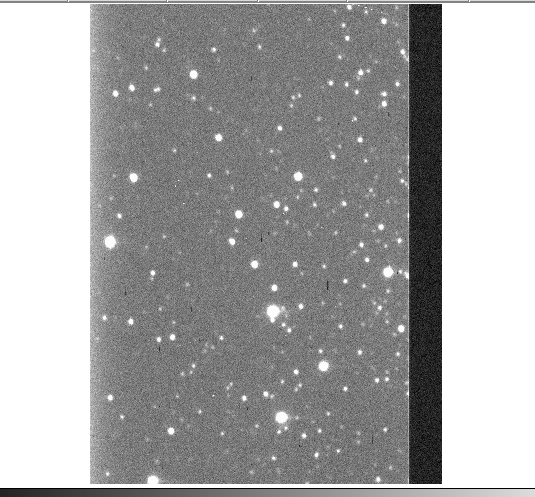
\includegraphics[width=0.5\linewidth]{Screenshot From 2026-07-06 14-04-23.png}
    \caption{Imagen m92010 en crudo}
    \label{fig:placeholder}
\end{figure}

\begin{figure}[H]
    \centering
    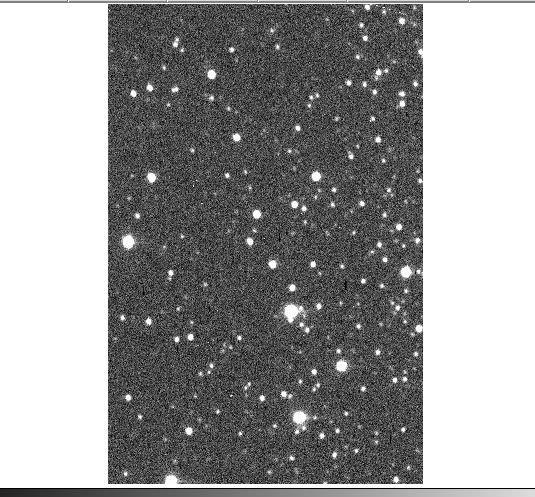
\includegraphics[width=0.5\linewidth]{Screenshot From 2026-07-06 14-06-10.png}
    \caption{Imagen m92010 reducida}
    \label{fig:placeholder}
\end{figure}

% ---------------------------------------------------------
\subsection{Taller 2: identificación manual de estrellas con \texttt{imexamine}}

En el segundo taller se trabajó con herramientas interactivas de IRAF para visualizar imágenes y seleccionar estrellas manualmente. Se usó \texttt{display} para cargar las imágenes en DS9 y \texttt{imexamine} para medir información sobre las estrellas seleccionadas. Esta parte permitió familiarizarse con el uso del cursor interactivo y con la interpretación de coordenadas, perfiles y estadísticas locales.

El procedimiento consistió en desplegar una imagen, ubicar estrellas relativamente brillantes y aisladas, y presionar teclas específicas dentro de \texttt{imexamine}. La tecla \texttt{a} permitió obtener información de la estrella bajo el cursor, incluyendo sus coordenadas. La tecla \texttt{r} permitió visualizar el perfil radial de una estrella, útil para estimar el FWHM. La tecla \texttt{m} permitió obtener estadísticas de una región, lo cual es útil para caracterizar el fondo de cielo.

\begin{lstlisting}
cl> display imagen.fits 1
cl> imexamine

# Dentro de la ventana de DS9:
# a  -> imprime información de la estrella
# r  -> muestra perfil radial
# m  -> muestra estadísticas locales
# x  -> imprime coordenadas
# q  -> salir
\end{lstlisting}

En este taller también se practicó la medición de posiciones de varias estrellas en diferentes imágenes. Esto permitió comparar desplazamientos entre imágenes y entender la importancia de seleccionar estrellas bien distribuidas sobre el campo.


% ---------------------------------------------------------
\subsection{Taller 3: fotometría de apertura en \texttt{m92011} y M41}

En el tercer taller se realizó fotometría de apertura. Esta etapa tuvo dos partes: primero se trabajó con una imagen de M92, principalmente \texttt{m92011}, y luego se aplicó el procedimiento al archivo \texttt{M41.fits}. En el caso de M41, el archivo era multiextensión y contenía tres canales: \texttt{blue}, \texttt{red} y \texttt{green}. Por esta razón, fue necesario separar las extensiones antes de aplicar las tareas de fotometría.

\subsubsection{Separación de canales en M41}

Al intentar visualizar directamente \texttt{M41.fits}, IRAF solicitó especificar la extensión FITS. Por ello se revisaron las extensiones disponibles y se crearon archivos independientes para cada canal:

\begin{lstlisting}
cl> imhead M41.fits[0] long+
cl> imhead M41.fits[1] long+
cl> imhead M41.fits[2] long+

cl> imcopy M41.fits[0] M41_blue.fits
cl> imcopy M41.fits[1] M41_red.fits
cl> imcopy M41.fits[2] M41_green.fits

cl> display M41_blue.fits 1
cl> display M41_red.fits 2
cl> display M41_green.fits 3
\end{lstlisting}

\begin{figure}[H]
    \centering
    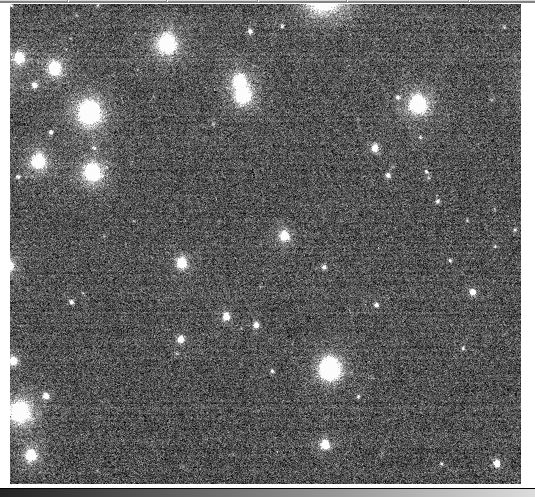
\includegraphics[width=0.5\linewidth]{Screenshot From 2026-07-06 14-13-44.png}
    \caption{imagen con filtro Blue de M41}
    \label{fig:placeholder}
\end{figure}

\begin{figure}[H]
    \centering
    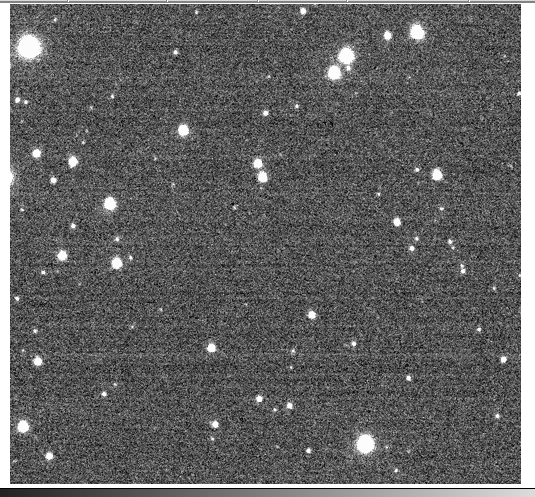
\includegraphics[width=0.5\linewidth]{Screenshot From 2026-07-06 14-13-55.png}
    \caption{imagen con filtro Red de M41}
    \label{fig:placeholder}
\end{figure}

\begin{figure}[H]
    \centering
    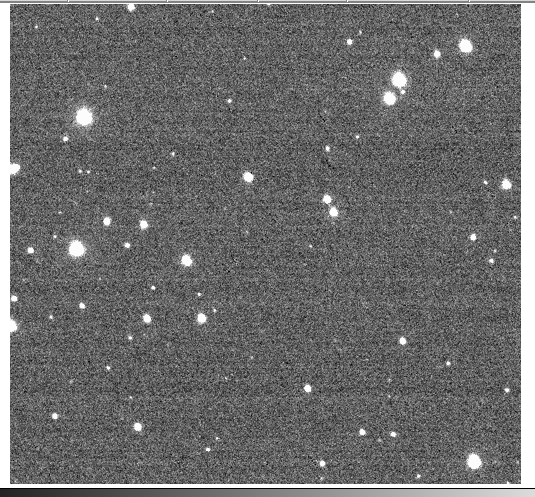
\includegraphics[width=0.5\linewidth]{Screenshot From 2026-07-06 14-14-03.png}
    \caption{imagen con filtro Green de M41}
    \label{fig:placeholder}
\end{figure}

\subsubsection{Medición de FWHM y fondo de cielo}

Antes de realizar la fotometría, se midió el FWHM de varias estrellas y se estimó el sigma del fondo de cielo. El FWHM se utilizó para definir el radio de apertura, mientras que el sigma del cielo fue necesario para evaluar la calidad de la detección de fuentes.

\begin{lstlisting}
cl> display m92011.fits 1
cl> imexamine m92011.fits

cl> display M41_green.fits 1
cl> imexamine M41_green.fits
\end{lstlisting}

\begin{table}[H]
    \centering
    \begin{tabular}{lccc}
        \toprule
        Imagen & Mediana del FWHM [pix] & Apertura usada $3\times$FWHM [pix] & Threshold \\
        \midrule
        \texttt{m92010.fits} & 2.900 & 8.700 & 3.5 \\
        \texttt{m92011.fits} & 3.355 & 10.065 & 3.5 \\
        \texttt{m92014.fits} & 3.295 & 9.885 & 3.5 \\
        \texttt{m92015.fits} & 3.025 & 9.075 & 3.5 \\
        \texttt{M41.fits}    & 2.220 & 6.660 & 3.5 \\
        \bottomrule
    \end{tabular}
    \caption{Valores de FWHM, apertura fotométrica y threshold utilizados para la detección y fotometría. La apertura se definió como tres veces la mediana del FWHM medido en cada imagen.}
    \label{tab:parametros_fwhm_threshold}
\end{table}

\subsubsection{Fotometría interactiva con \texttt{qphot}}

Para la imagen \texttt{m92011}, se realizó fotometría de apertura usando \texttt{qphot}. Esta tarea permitió medir estrellas seleccionadas y obtener magnitudes instrumentales junto con sus errores.

\begin{lstlisting}
cl> digiphot
cl> apphot

cl> display m92011.fits 1
cl> epar qphot

# Parámetros usados:
# cbox     = 5 o 7
# annulus  = 15
# dannulus = 10
# apertures = 10
# interactive = yes

cl> qphot m92011.fits
\end{lstlisting}

Después de obtener el archivo de salida, se extrajeron las columnas principales:

\begin{lstlisting}
cl> txdump m92011.mag.1 xcenter,ycenter,mag,merr yes > m92011_qphot.dat
\end{lstlisting}


\subsubsection{Detección automática y fotometría en M41}

Para M41 se aplicó una detección automática de estrellas con \texttt{daofind}. Se probaron varios valores de \texttt{threshold} para escoger el mejor compromiso entre detectar estrellas débiles y evitar falsas detecciones. Luego se revisaron las coordenadas con \texttt{tvmark} y se ejecutó la fotometría con \texttt{phot}.

\begin{lstlisting}
cl> daofind M41_green.fits output=M41_green.coo \
    fwhmpsf=FWHM sigma=SIGMA threshold=THRESHOLD verify-

cl> display M41_green.fits 1
cl> tvmark 1 coords=M41_green.coo mark=circle radii=5 color=204 number+

cl> phot M41_green.fits coords=M41_green.coo output=M41_green.mag interac- verify-

cl> txdump M41_green.mag XCENTER,YCENTER,MAG,MERR yes > M41_green.dat
\end{lstlisting}

Para contar el número de estrellas detectadas en el archivo \texttt{.coo}, se exportaron las coordenadas y se contaron las líneas:

\begin{lstlisting}
cl> txdump M41_green.coo XCENTER,YCENTER,ID yes > M41_green.xy
cl> !wc -l M41_green.xy
\end{lstlisting}

\begin{figure}[H]
    \centering
    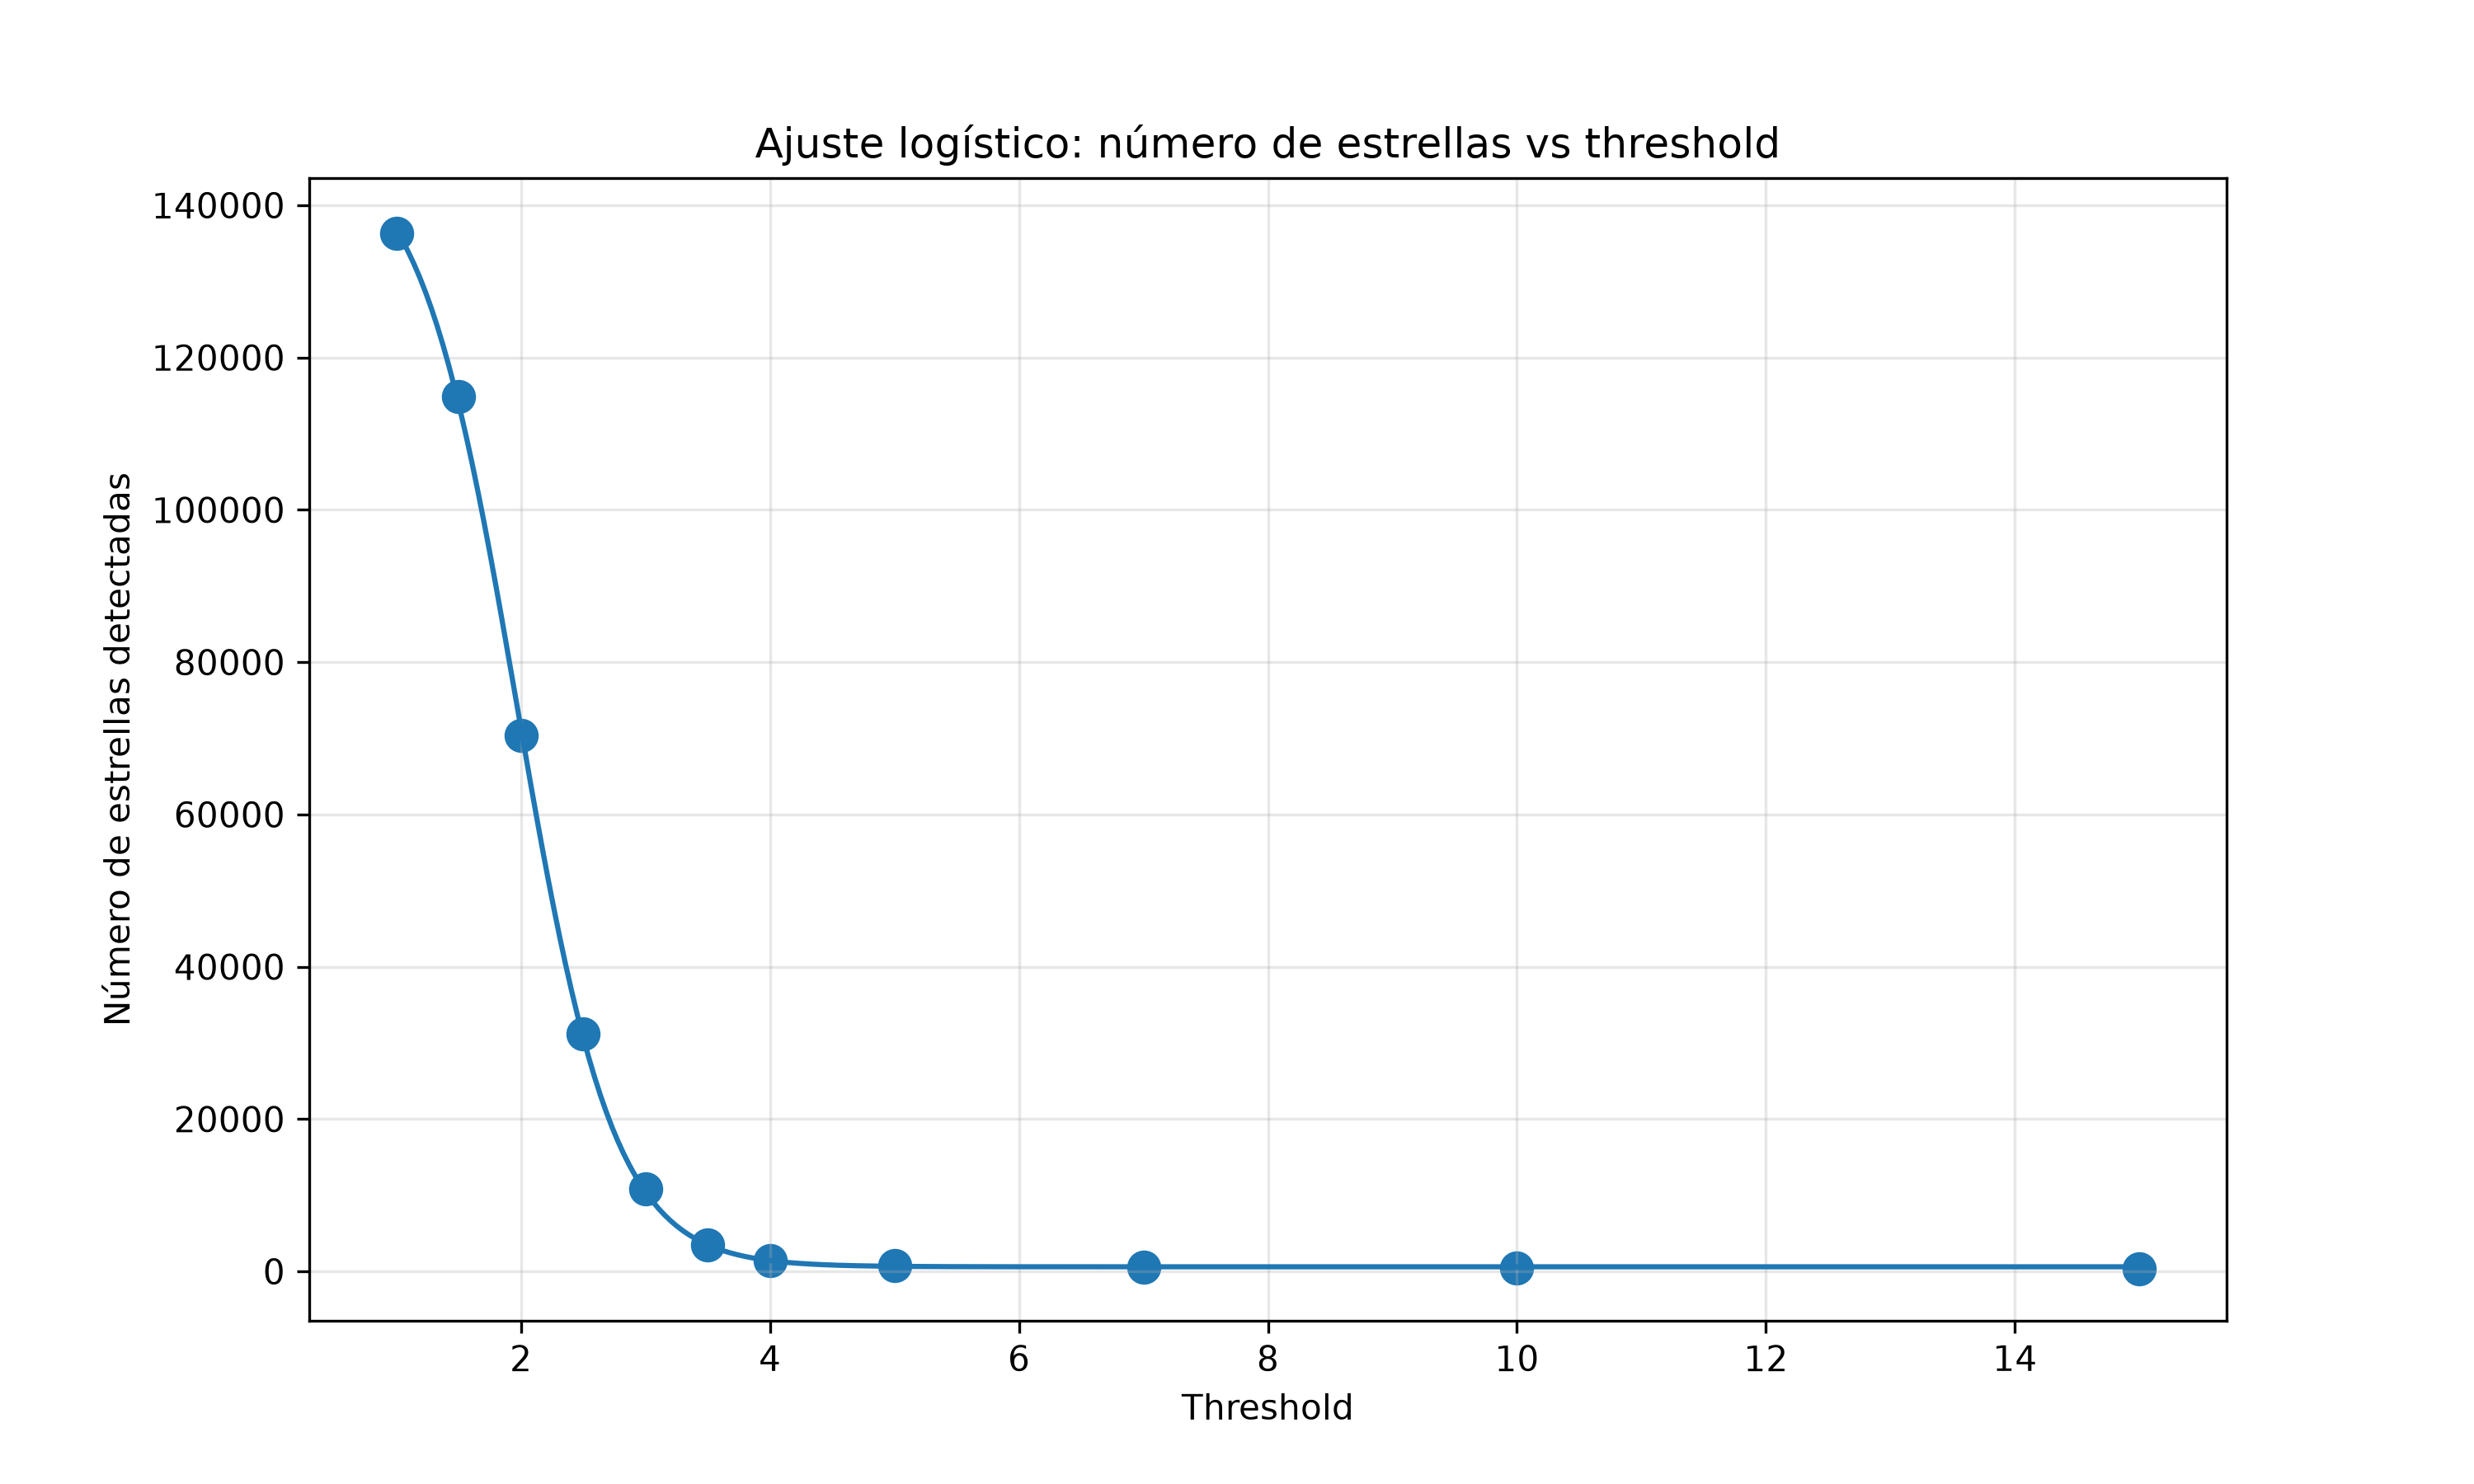
\includegraphics[width=0.8\linewidth]{ajuste_logistico.png}
    \caption{ajuste para encontrar el numero de thersholds a usar para M41}
    \label{fig:placeholder}
\end{figure}

\begin{figure}[H]
    \centering
    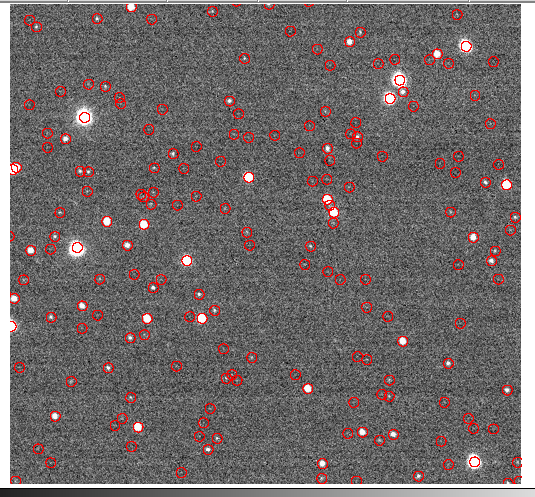
\includegraphics[width=0.5\linewidth]{Screenshot From 2026-07-06 14-19-30.png}
    \caption{Estrellas encontradas en la imagen M41}
    \label{fig:placeholder}
\end{figure}

\subsubsection{Detección automática y fotometría en M92}

Para la imagen \texttt{m92011.fits} se realizó una detección automática de estrellas mediante \texttt{daofind}. El objetivo fue obtener una lista inicial de coordenadas de fuentes estelares para posteriormente realizar fotometría de apertura y construir el diagrama color-magnitud de M92.

En esta etapa se utilizó un valor de \texttt{threshold} igual a 3.5, ya que permitió detectar una cantidad amplia de estrellas sin aumentar excesivamente las falsas detecciones. Además, se empleó el valor mediano del FWHM medido previamente para la imagen \texttt{m92011.fits}.

\begin{figure}[H]
    \centering
    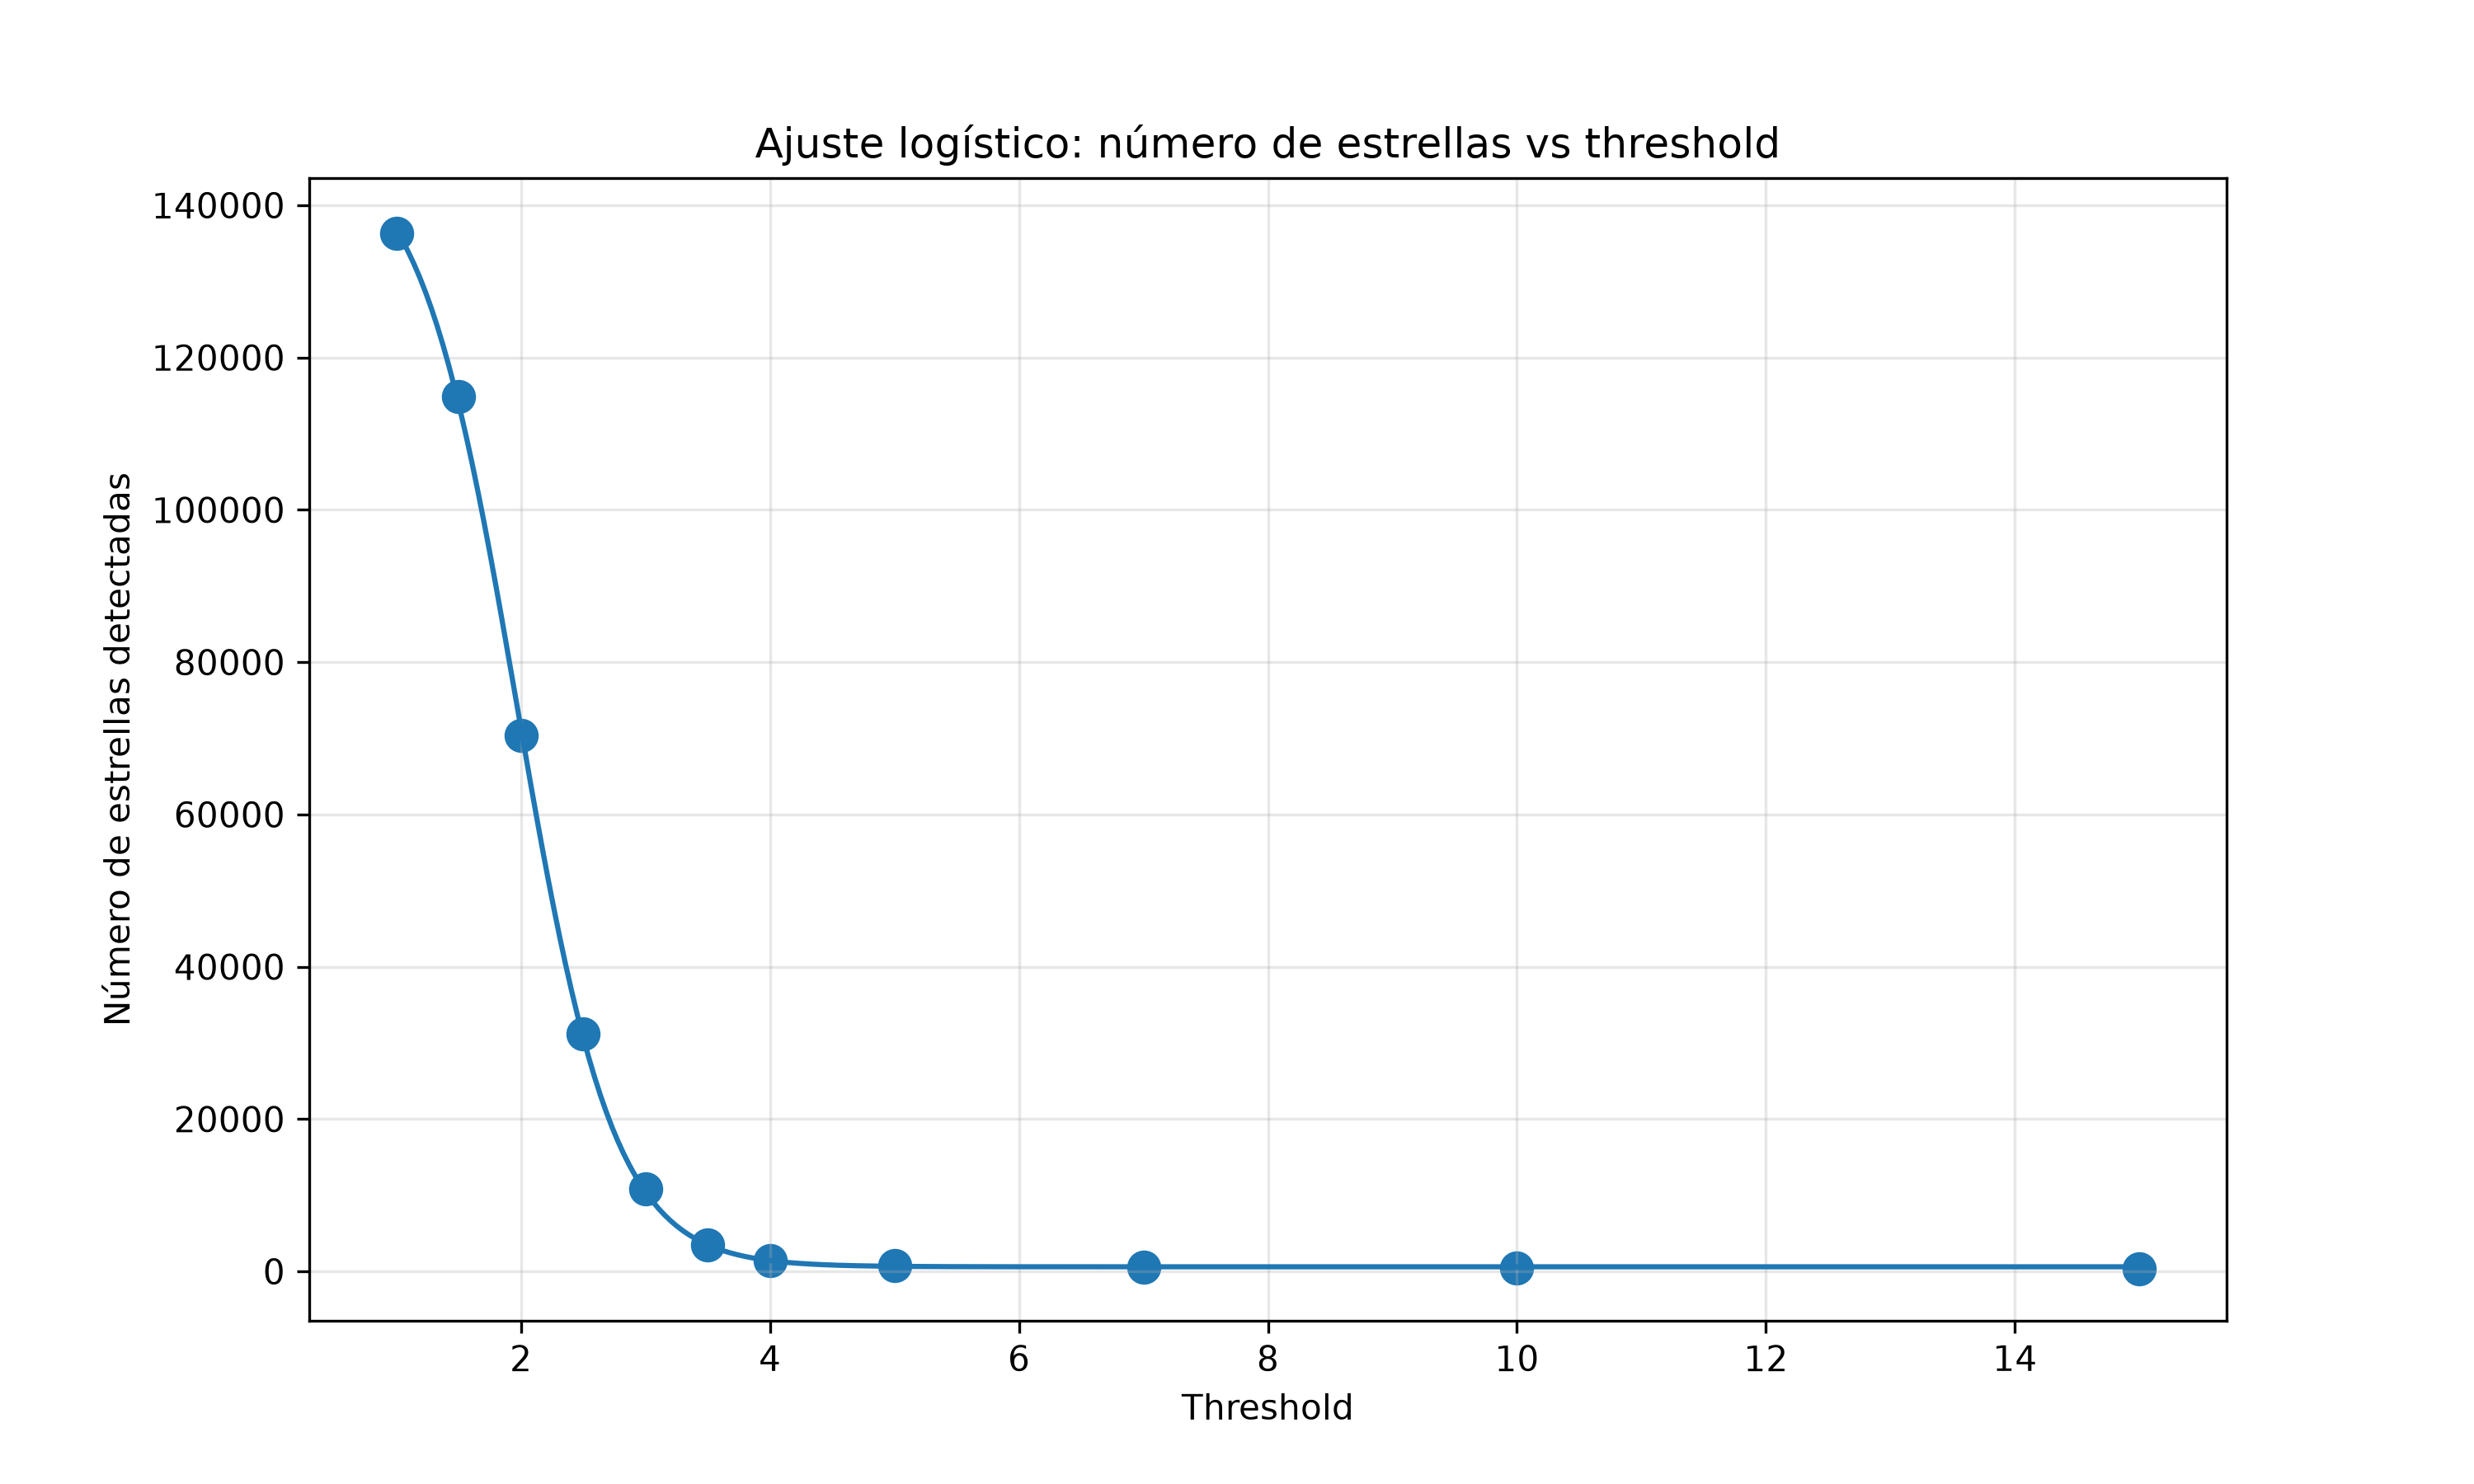
\includegraphics[width=0.8\linewidth]{ajuste_logistico.png}
    \caption{ajuste para encontrar el numero de thersholds a usar para M92}
    \label{fig:placeholder}
\end{figure}

\begin{figure}[H]
    \centering
    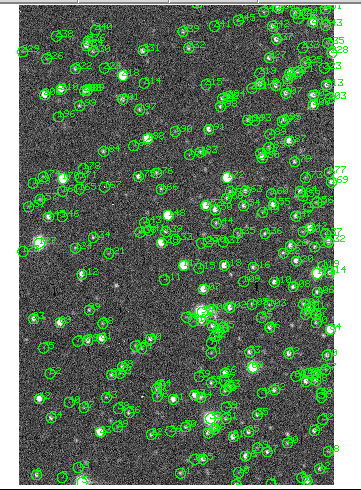
\includegraphics[width=0.5\linewidth]{Screenshot From 2026-07-13 13-19-04.png}
    \caption{Estrellas detectadas automáticamente en la imagen \texttt{m92011.fits} de M92 usando \texttt{daofind} con un \texttt{threshold} de 3.5.}
    \label{fig:m92011_estrellas_detectadas}
\end{figure}

\subsubsection{Gráficas de magnitud contra error}

Después de obtener las magnitudes instrumentales mediante fotometría de apertura, se construyeron gráficas de magnitud contra error fotométrico. Estas gráficas permiten evaluar la calidad de las mediciones, ya que se espera que las estrellas más brillantes presenten errores menores, mientras que las estrellas más débiles tengan errores más altos debido a una menor relación señal-ruido.

\begin{figure}[H]
    \centering
    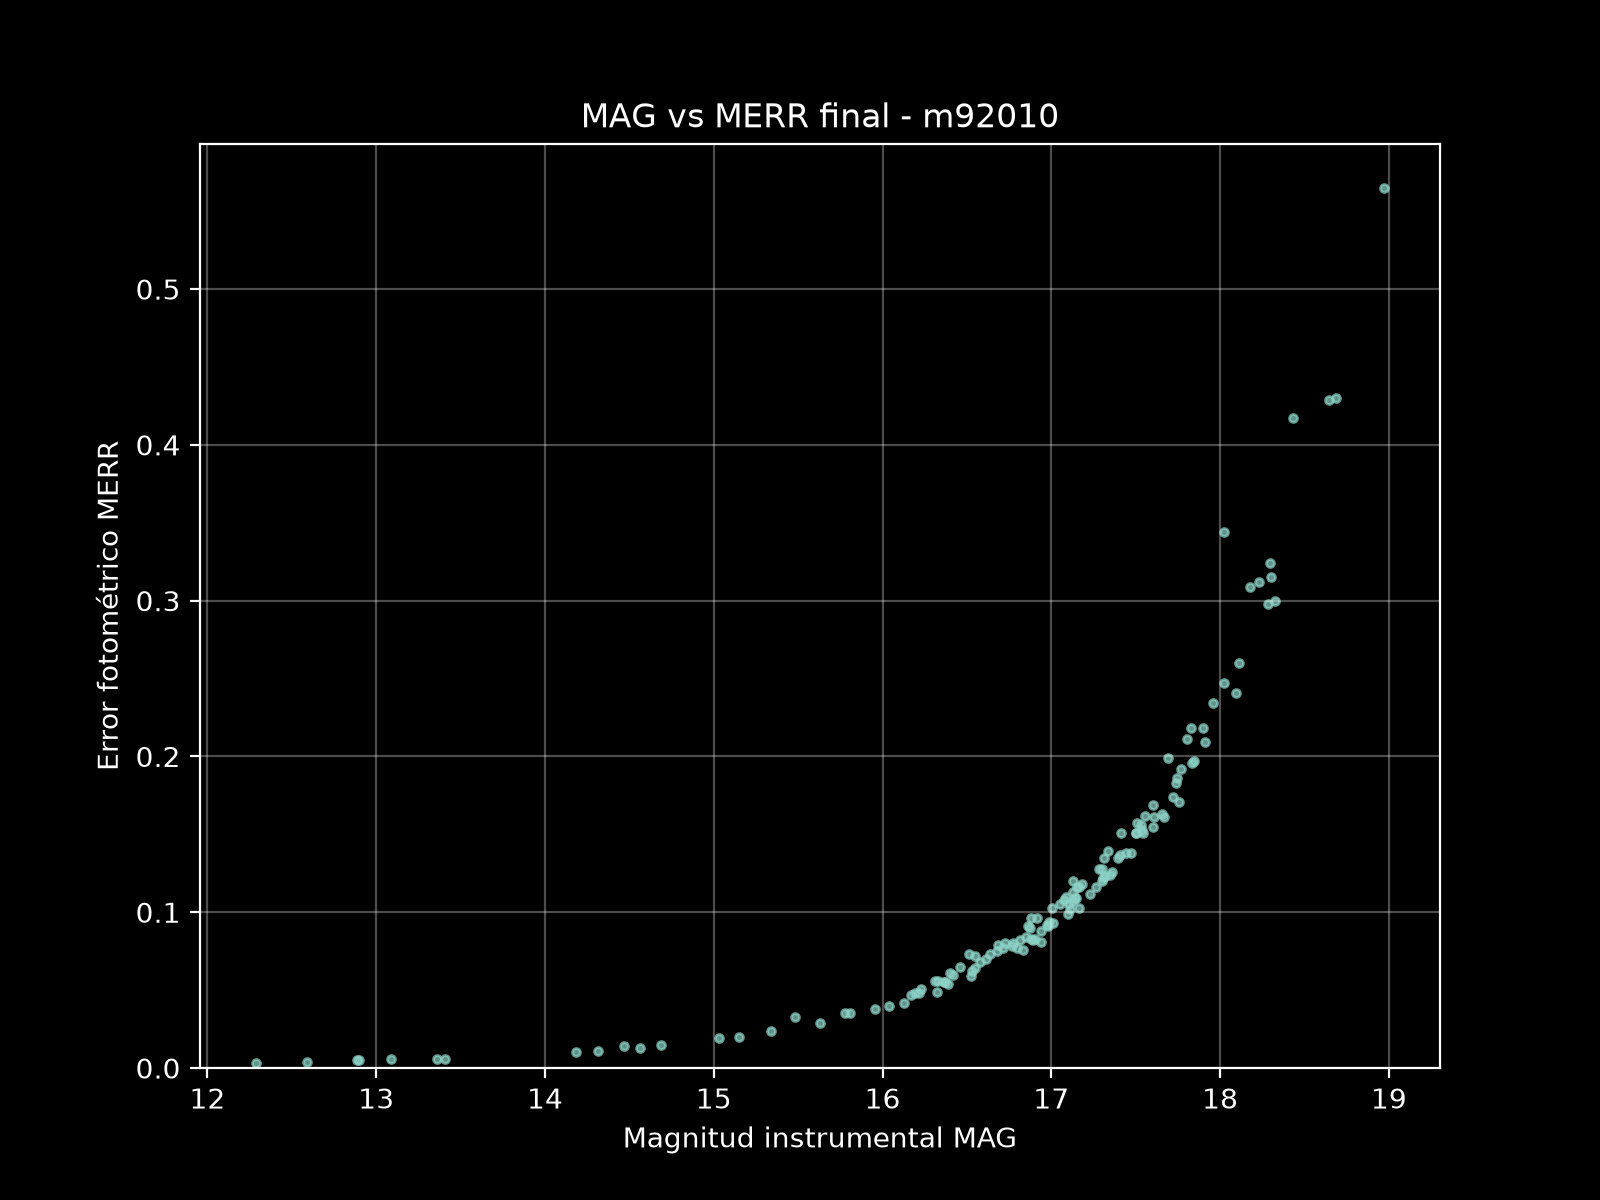
\includegraphics[width=0.5\linewidth]{m92010_final_mag_vs_merr.png}
    \caption{Gráfica de magnitud instrumental contra error fotométrico para la imagen \texttt{m92010.fits}.}
    \label{fig:m92010_mag_merr}
\end{figure}

\begin{figure}[H]
    \centering
    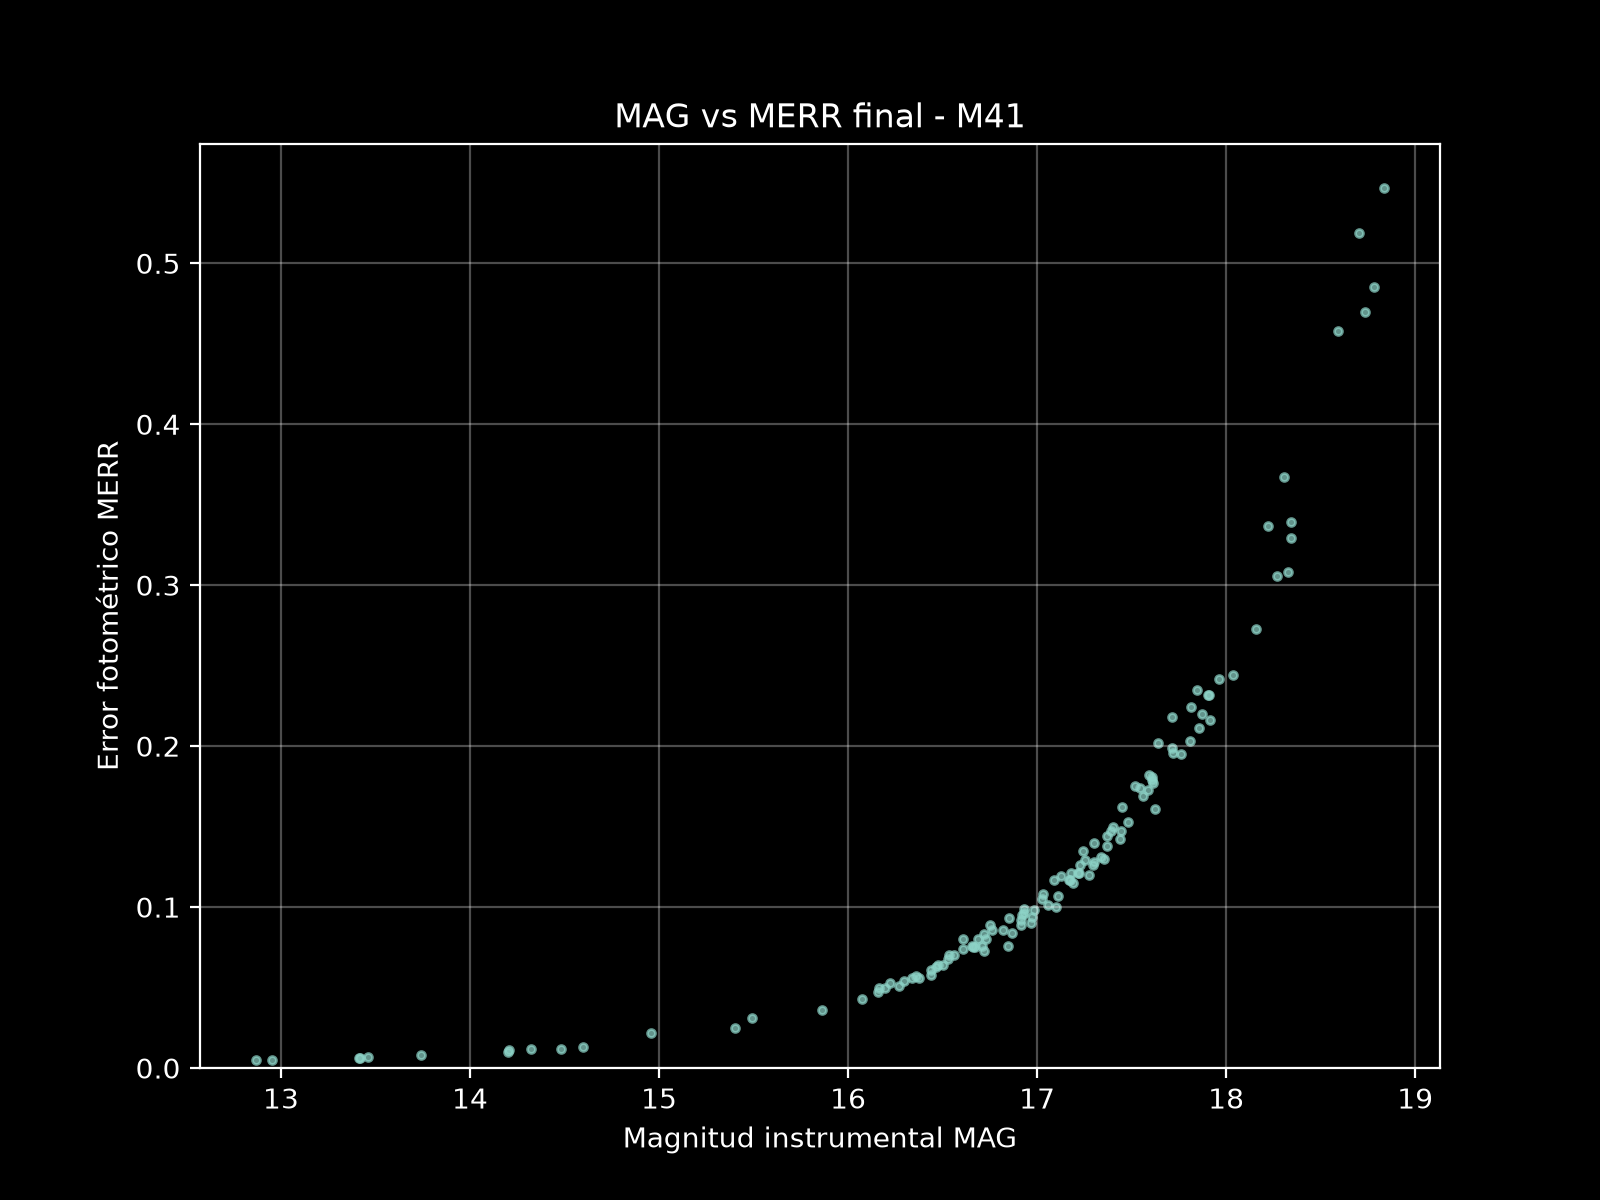
\includegraphics[width=0.5\linewidth]{m91_final_mag_vs_merr.png}
    \caption{Gráfica de magnitud instrumental contra error fotométrico para M41.}
    \label{fig:m41_mag_merr}
\end{figure}

Cabe aclarar que se utilizaron los valores reportados en los repositorios:

\href{https://github.com/sserranop1/LAB.5}{Repositorio del trabajo realizado sobre M92}

\href{https://github.com/sserranop1/M41}{Repositorio del trabajo realizado sobre M41}

\subsubsection{CMD de M92}

A partir de los resultados de la fotometría en los filtros $B$ y $V$, se construyó el diagrama color-magnitud instrumental de M92. Para esto se utilizaron las imágenes \texttt{m92011.fits} y \texttt{m92015.fits}. La imagen \texttt{m92011.fits} fue tomada como el filtro $V$, mientras que \texttt{m92015.fits} fue tomada como el filtro $B$.

El color instrumental se calculó como:

\[
B - V = m_B - m_V,
\]

donde $m_B$ corresponde a la magnitud instrumental medida en el filtro $B$ y $m_V$ corresponde a la magnitud instrumental medida en el filtro $V$. Luego se graficó el color $B-V$ en el eje horizontal y la magnitud instrumental $V$ en el eje vertical. El eje vertical fue invertido siguiendo la convención astronómica, en la cual las magnitudes menores corresponden a objetos más brillantes.

\begin{figure}[H]
    \centering
    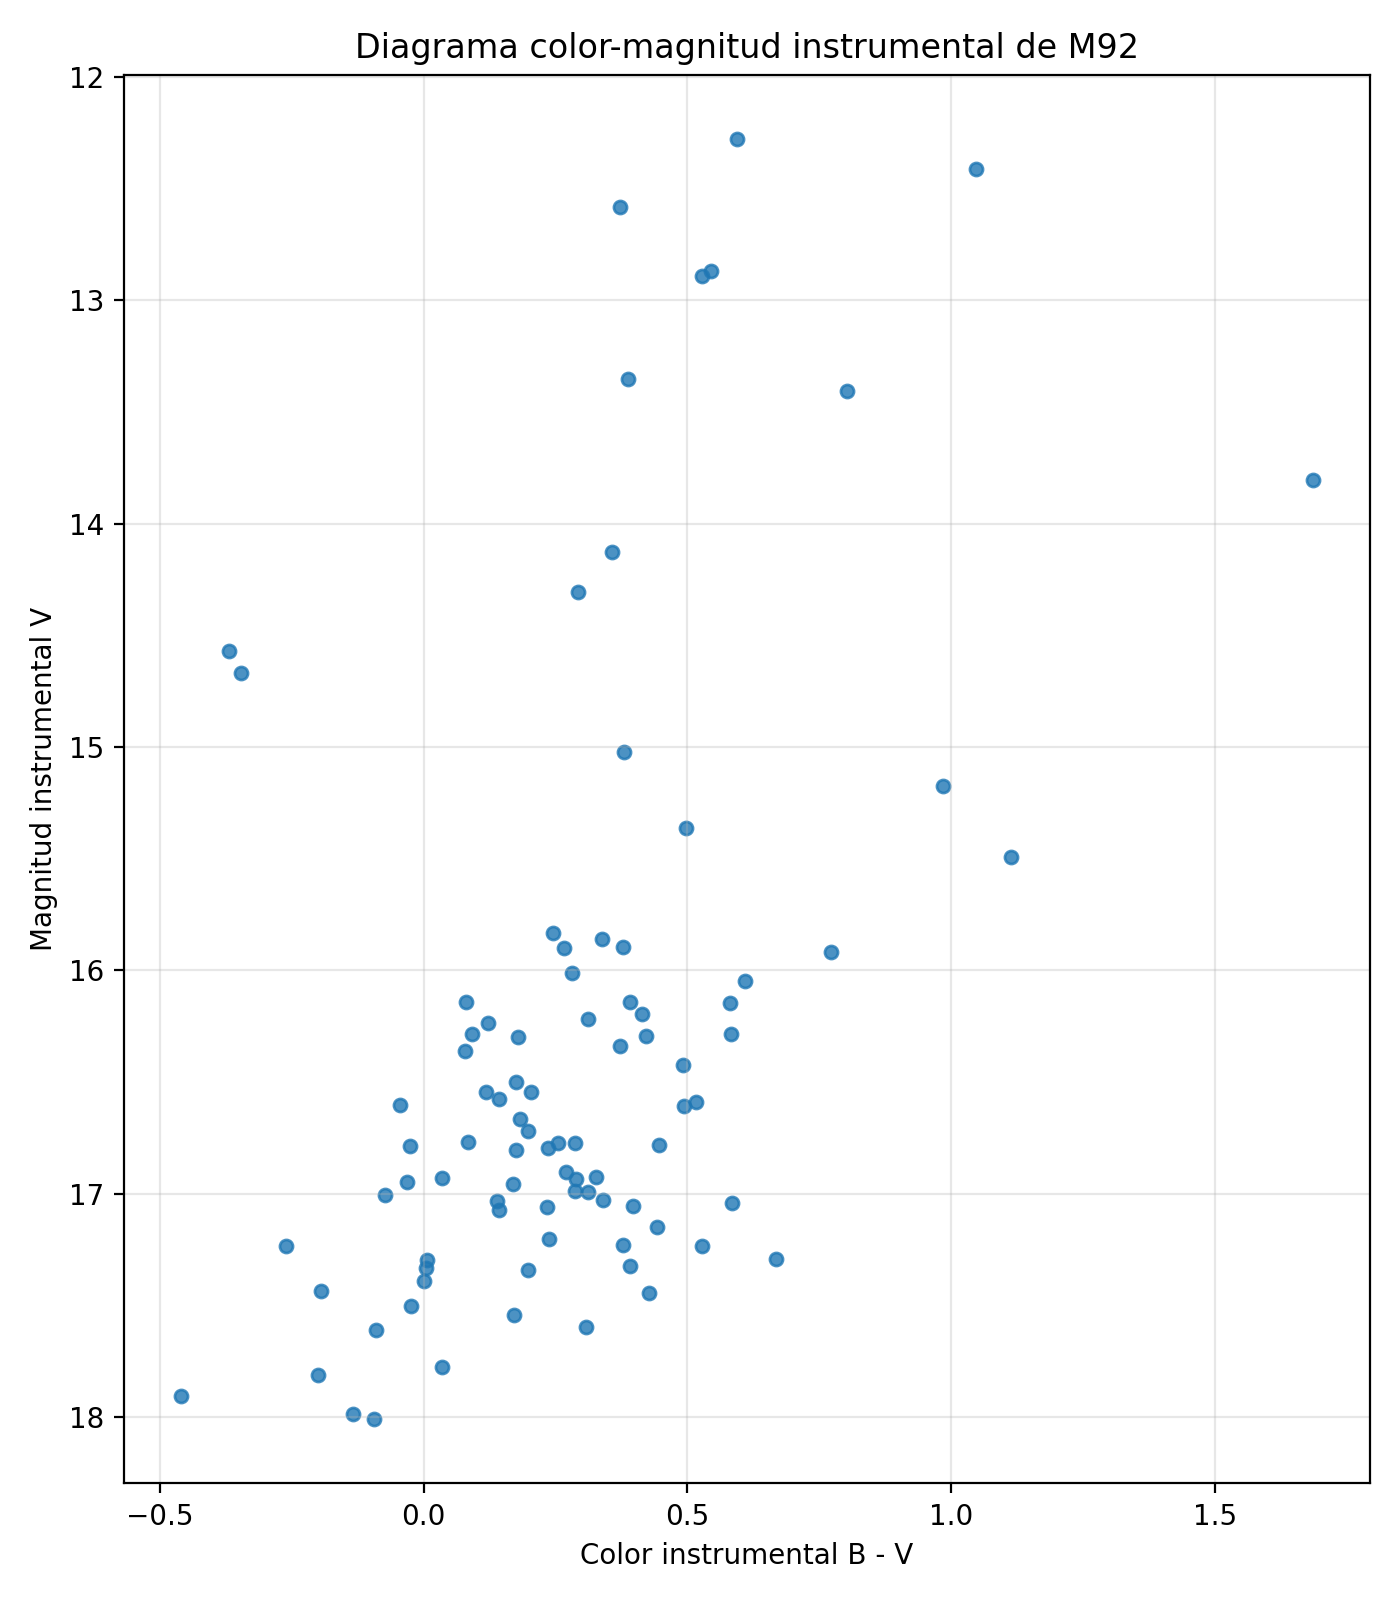
\includegraphics[width=0.5\linewidth]{M92_CMD_clean.png}
    \caption{Diagrama color-magnitud instrumental de M92 construido a partir de las imágenes \texttt{m92011.fits} y \texttt{m92015.fits}. En el eje horizontal se muestra el color instrumental $B-V$ y en el eje vertical la magnitud instrumental $V$.}
    \label{fig:cmd_m92}
\end{figure}

\subsubsection{Criterio de aislamiento por vecinos más cercanos en M92}

Después de construir una primera muestra fotométrica para el CMD, se aplicó un criterio adicional de filtrado para seleccionar únicamente fuentes suficientemente aisladas. Este paso fue necesario porque, en campos estelares densos, una estrella cercana puede contaminar la apertura fotométrica de otra fuente y afectar la medición de su magnitud instrumental.

Para cada estrella detectada se calculó la distancia euclidiana a su vecino más cercano usando sus coordenadas $(x,y)$. El criterio adoptado fue descartar toda estrella cuya fuente más cercana estuviera a una distancia menor o igual a $3\times FWHM$. En el caso de la imagen \texttt{m92011.fits}, el valor mediano del FWHM fue de 3.355 píxeles, por lo que el radio de exclusión utilizado fue:

\[
3\times FWHM = 3 \times 3.355 = 10.065 \text{ píxeles}.
\]

Por lo tanto, si una estrella tenía otra fuente dentro de un radio de 10.065 píxeles, fue clasificada como rechazada por posible contaminación fotométrica. En cambio, si su vecino más cercano estaba por fuera de este radio, la estrella fue considerada aceptada para el análisis.

Con este procedimiento se obtuvieron dos listas de coordenadas: una correspondiente a las estrellas aceptadas por estar suficientemente aisladas y otra correspondiente a las estrellas rechazadas por tener una fuente vecina dentro del radio de exclusión. Posteriormente, ambas listas fueron marcadas sobre la imagen usando \texttt{tvmark}, con el fin de verificar visualmente el resultado del filtrado.

\begin{figure}[H]
    \centering
    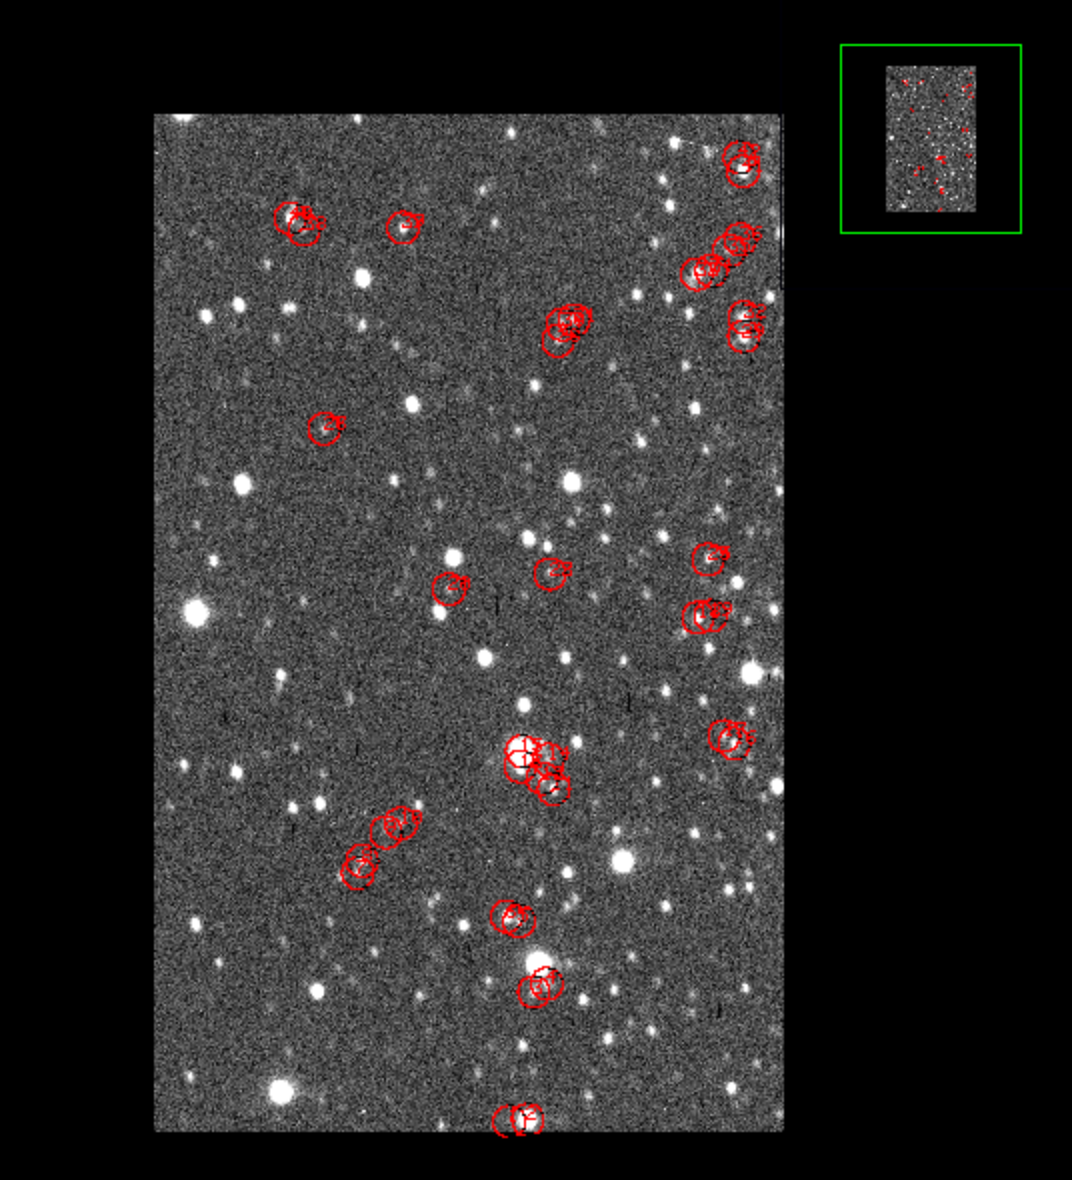
\includegraphics[width=0.6\linewidth]{Captura de pantalla 2026-07-14 a la(s) 5.42.51 p.m..png}
    \caption{Estrellas rechazadas en la imagen \texttt{m92011.fits} por presentar un vecino más cercano dentro de un radio de $3\times FWHM$. Estas fuentes no fueron consideradas para el análisis fotométrico final debido a la posible contaminación producida por estrellas cercanas. Se rechazaron 14 estrellas.}
    \label{fig:m92011_rechazadas_vecinos}
\end{figure}

\begin{figure}[H]
    \centering
    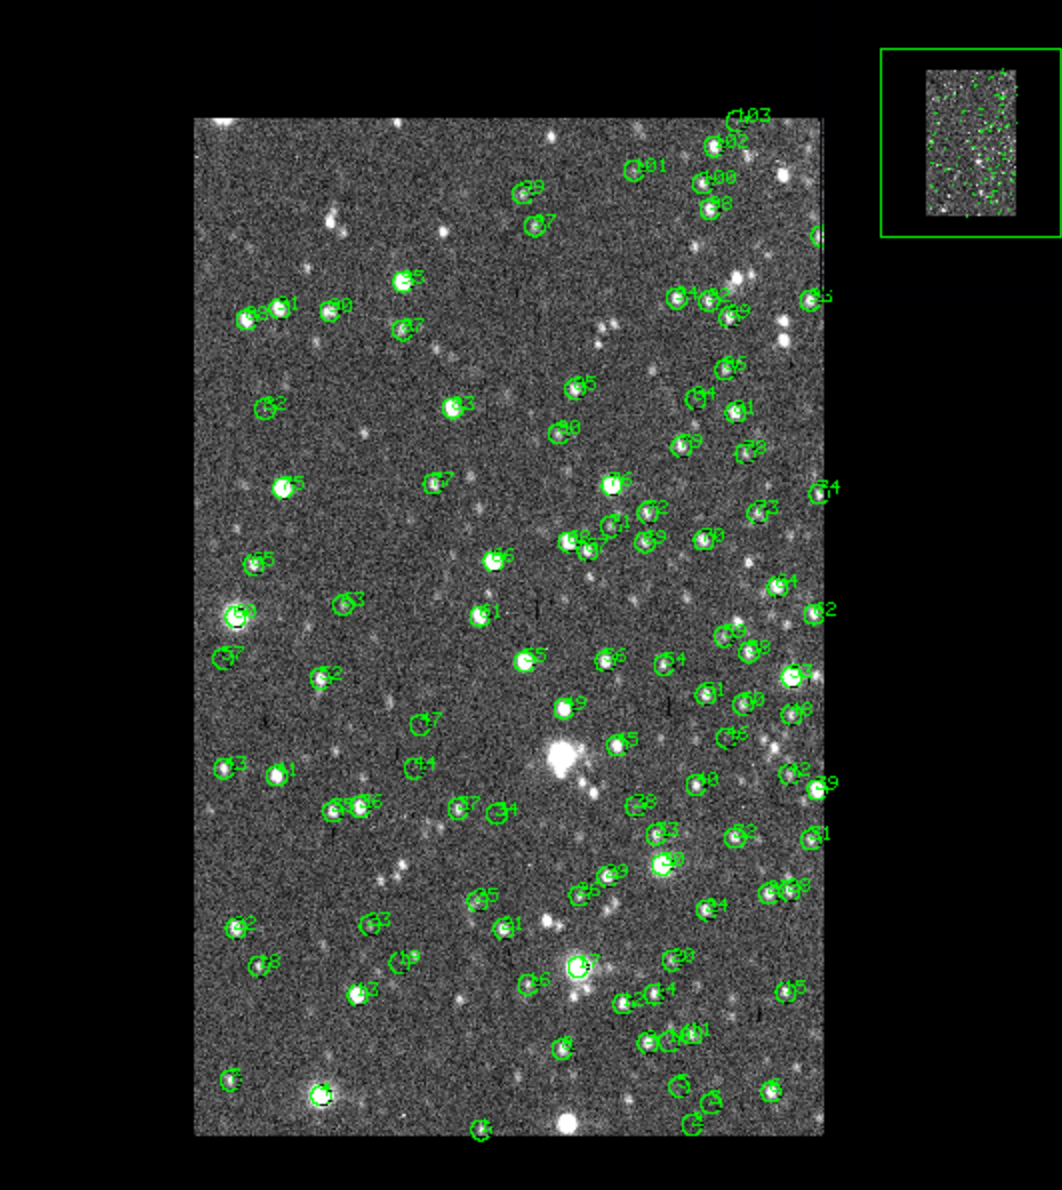
\includegraphics[width=0.6\linewidth]{Captura de pantalla 2026-07-14 a la(s) 5.43.18 p.m..png}
    \caption{Estrellas aceptadas en la imagen \texttt{m92011.fits} después de aplicar el criterio de aislamiento. Estas fuentes tienen su vecino más cercano a una distancia mayor que $3\times FWHM$, por lo que son más adecuadas para la fotometría de apertura.}
    \label{fig:m92011_aceptadas_vecinos}
\end{figure}

Este filtrado permitió mejorar la selección de estrellas utilizadas en la fotometría, reduciendo el efecto de fuentes mezcladas o demasiado cercanas. De esta manera, las magnitudes instrumentales obtenidas para las estrellas aceptadas son más confiables, ya que la apertura fotométrica tiene menor probabilidad de incluir flujo proveniente de una estrella vecina.

\subsubsection{Revisión de contaminación en los anillos de cielo}

Además del criterio de aislamiento por vecinos más cercanos, se revisó la posible contaminación dentro de los anillos de cielo utilizados para estimar el fondo local de cada estrella. En fotometría de apertura, el anillo de cielo debe representar únicamente el fondo local alrededor de la fuente. Sin embargo, si dentro de este anillo cae otra estrella, el valor estimado del cielo puede aumentar artificialmente y afectar la magnitud instrumental obtenida.

Para evaluar este efecto, se extrajeron los valores de los píxeles contenidos dentro del anillo de cielo de cada estrella en la imagen \texttt{m92011.fits}. Posteriormente, se construyó un diagrama de caja para analizar la distribución de cuentas en cada anillo. La presencia de valores atípicos altos puede indicar que el anillo contiene píxeles asociados a otra fuente estelar y no solamente al fondo de cielo.

En este análisis se utilizaron los mismos parámetros de fotometría definidos previamente: un radio interno del anillo de cielo de 15 píxeles y un ancho de anillo de 10 píxeles. Por tanto, el anillo de cielo se extendió desde 15 hasta 25 píxeles alrededor del centro de cada estrella.

\begin{figure}[H]
    \centering
    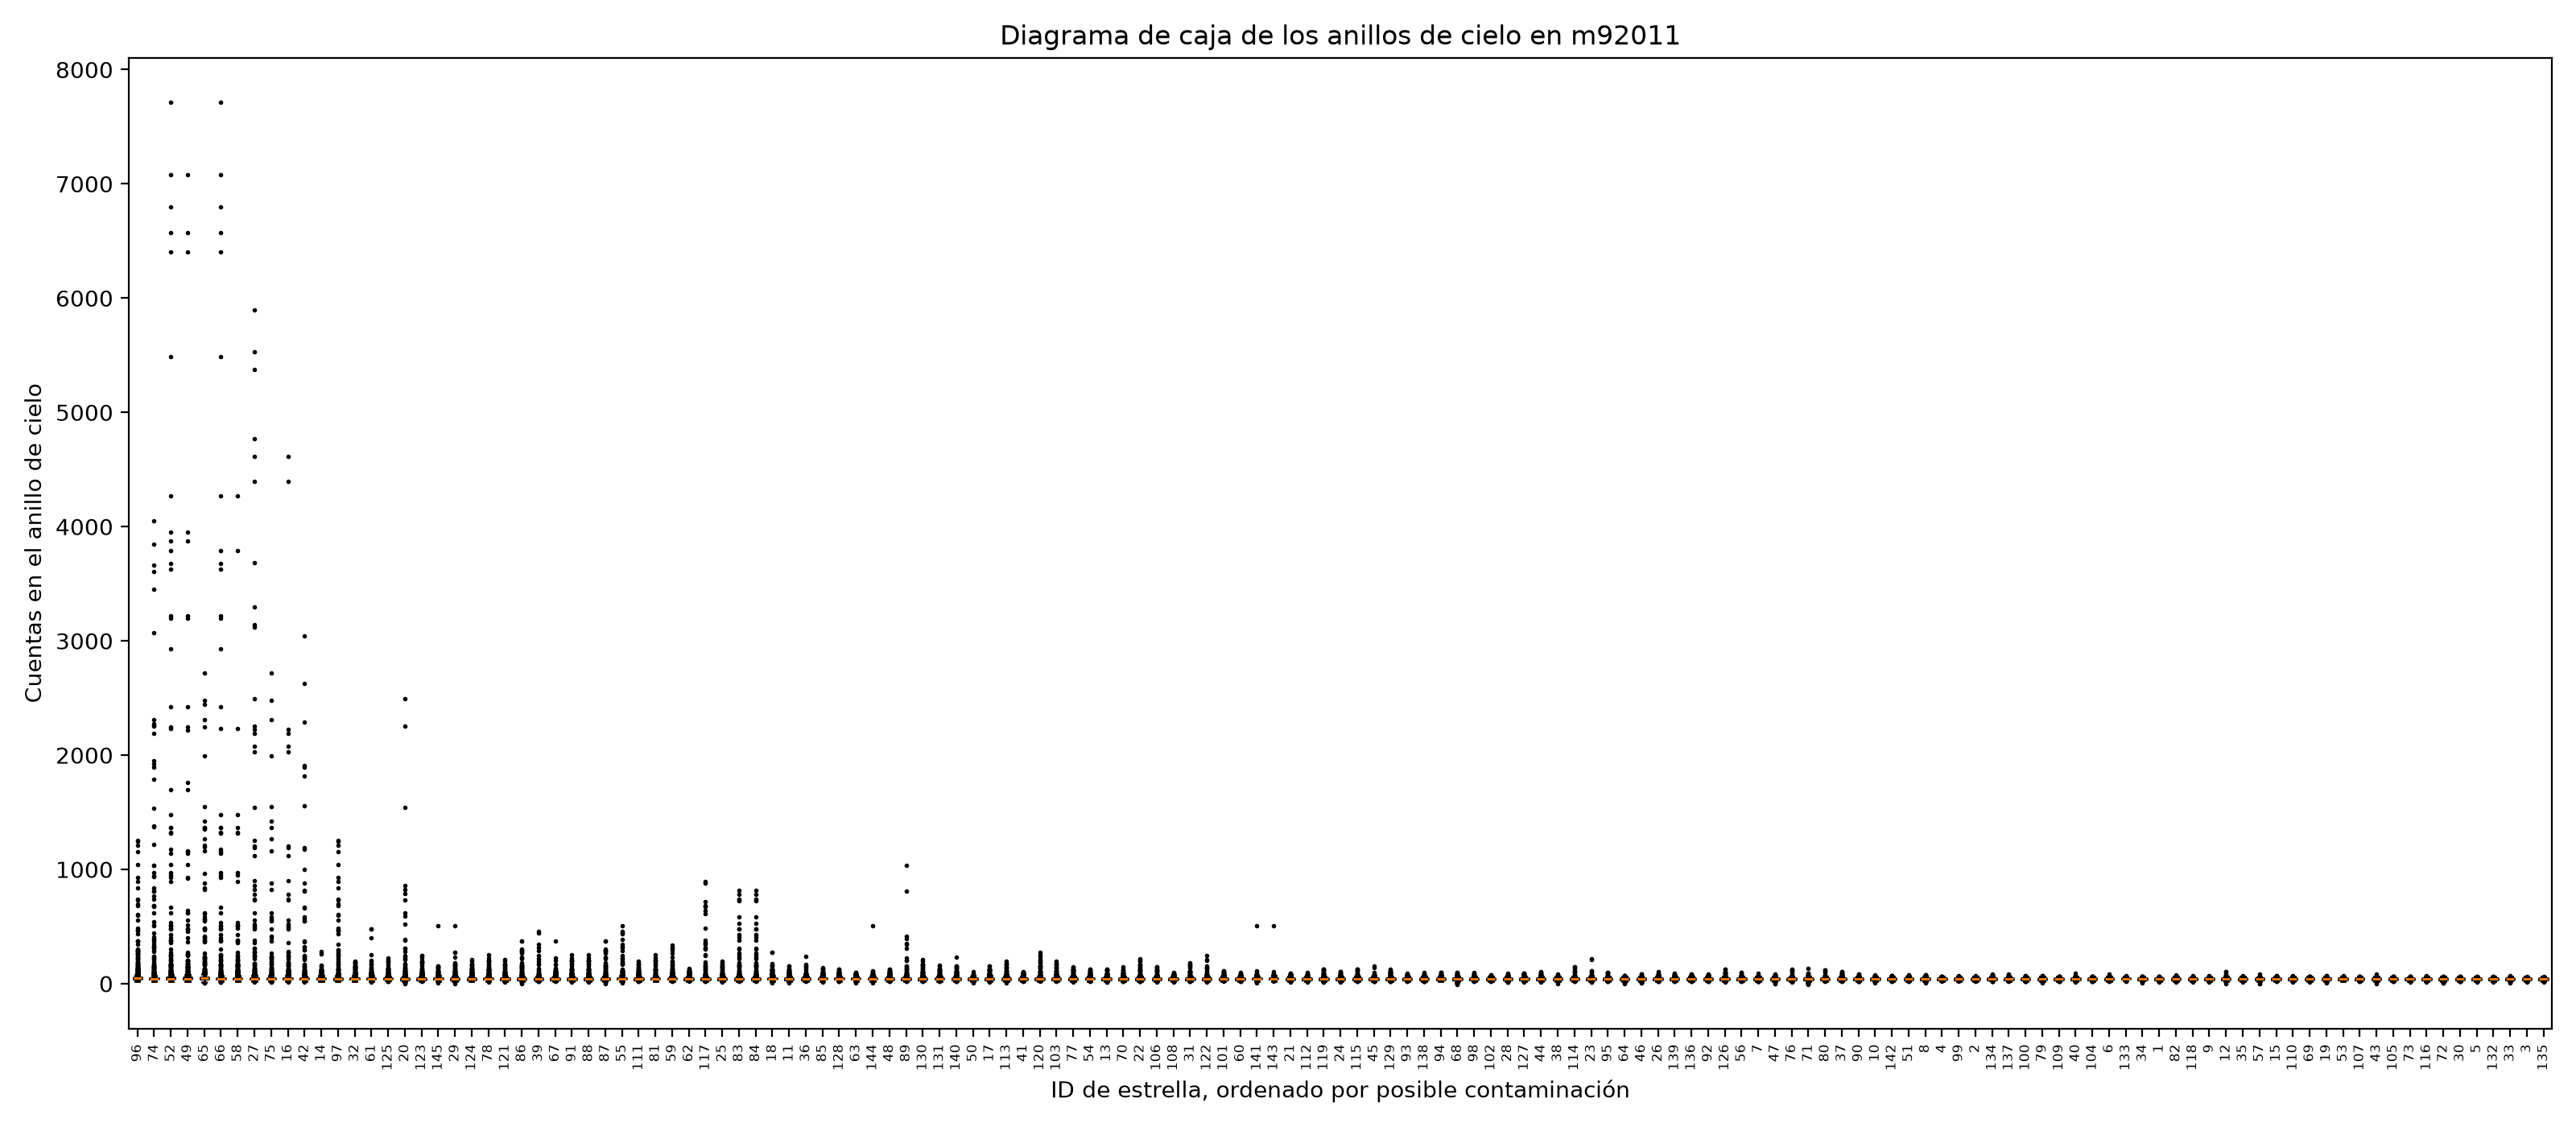
\includegraphics[width=0.9\linewidth]{m92011_boxplot_anillos_cielo.png}
    \caption{Diagrama de caja de los valores de píxeles en los anillos de cielo de las estrellas detectadas en \texttt{m92011.fits}. Los valores atípicos altos pueden indicar contaminación del anillo por fuentes cercanas.}
    \label{fig:boxplot_anillos_m92011}
\end{figure}

También se calculó la fracción de píxeles atípicos altos en cada anillo de cielo. Las estrellas cuyo anillo presentaba una fracción elevada de valores atípicos fueron clasificadas como rechazadas, debido a que su estimación del fondo podía estar contaminada por otra estrella.

\begin{figure}[H]
    \centering
    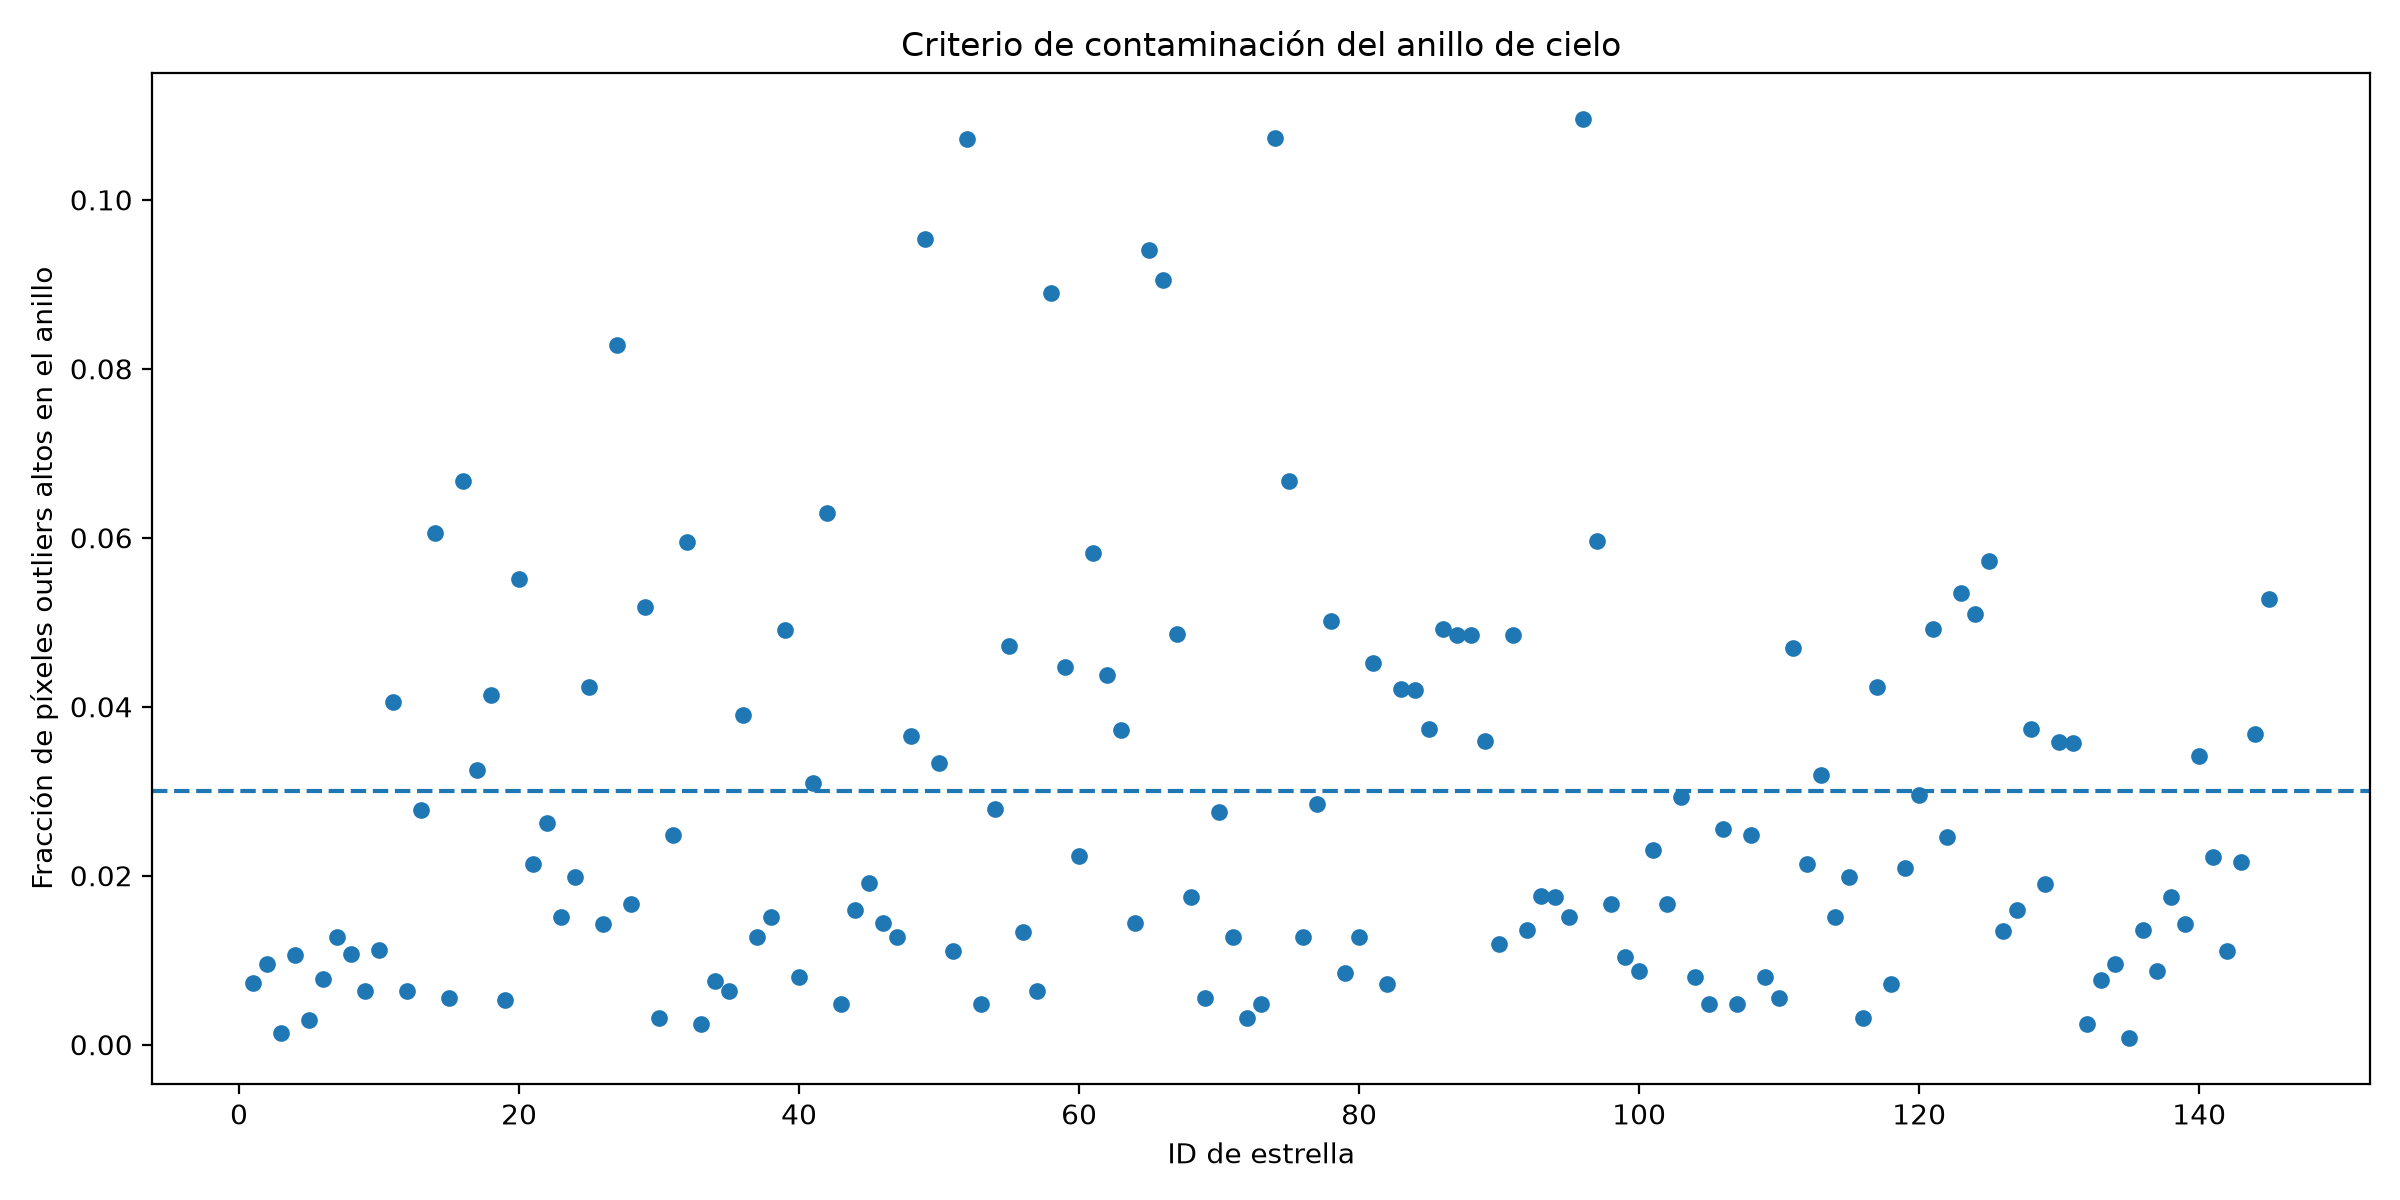
\includegraphics[width=0.8\linewidth]{m92011_outliers_anillos_cielo.png}
    \caption{Fracción de píxeles atípicos altos en el anillo de cielo de cada estrella. La línea punteada representa el límite usado para identificar anillos posiblemente contaminados.}
    \label{fig:outliers_anillos_m92011}
\end{figure}

Las estrellas rechazadas por este criterio fueron marcadas visualmente sobre la imagen con \texttt{tvmark}. Esto permitió verificar si las fuentes descartadas correspondían efectivamente a casos donde el anillo de cielo podía incluir flujo proveniente de estrellas cercanas.

\begin{figure}[H]
    \centering
    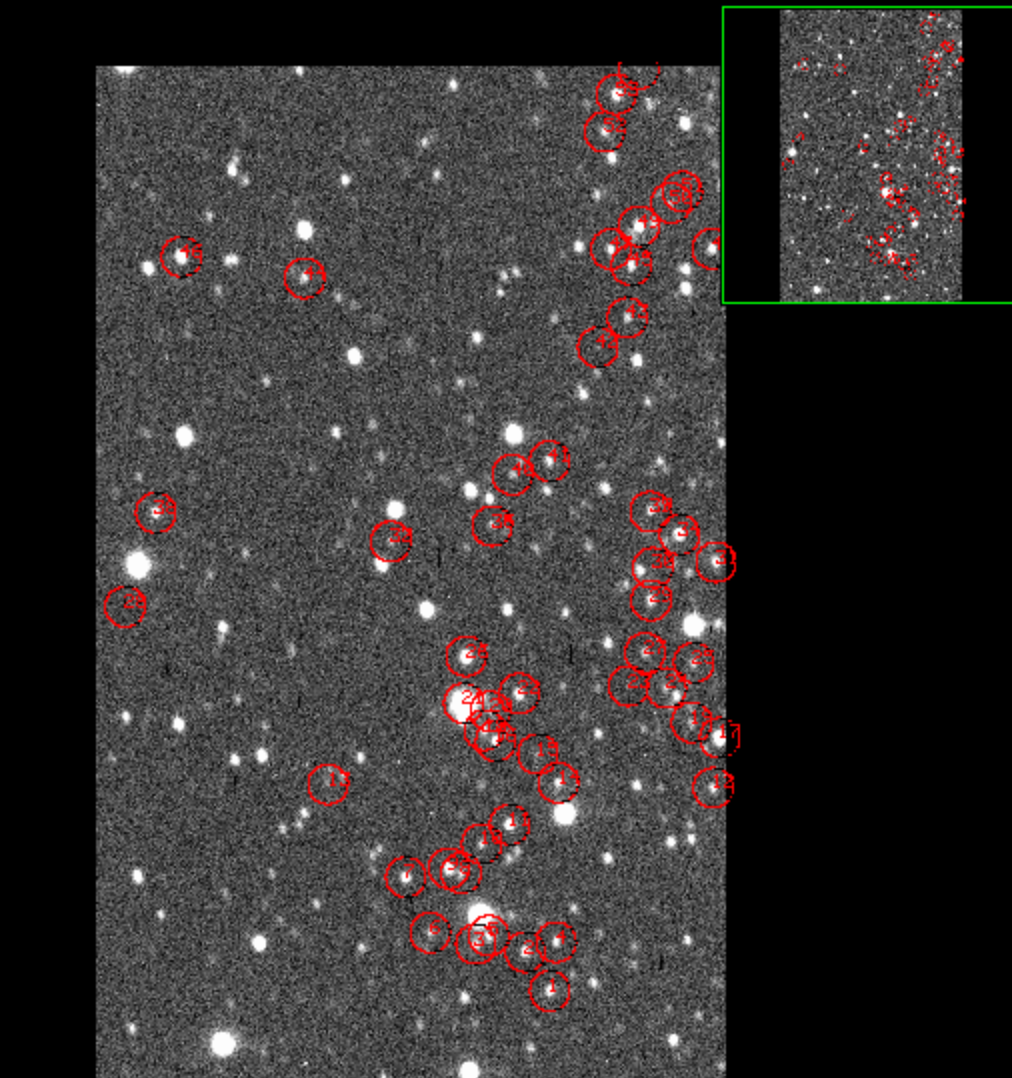
\includegraphics[width=0.6\linewidth]{Captura de pantalla 2026-07-14 a la(s) 5.58.18 p.m..png}
    \caption{Estrellas rechazadas en \texttt{m92011.fits} porque su anillo de cielo presentó indicios de contaminación por fuentes cercanas, se rechazaron 28 estrellas.}
    \label{fig:rechazadas_anillo_m92011}
\end{figure}

Este procedimiento permitió depurar aún más la muestra fotométrica, eliminando estrellas cuya medición podía verse afectada por una mala estimación del fondo local. De esta forma, las estrellas conservadas para el análisis final cumplen tanto el criterio de aislamiento como el criterio de anillo de cielo no contaminado.

Las estrellas aceptadas fueron las siguientes:

\begin{figure}[H]
    \centering
    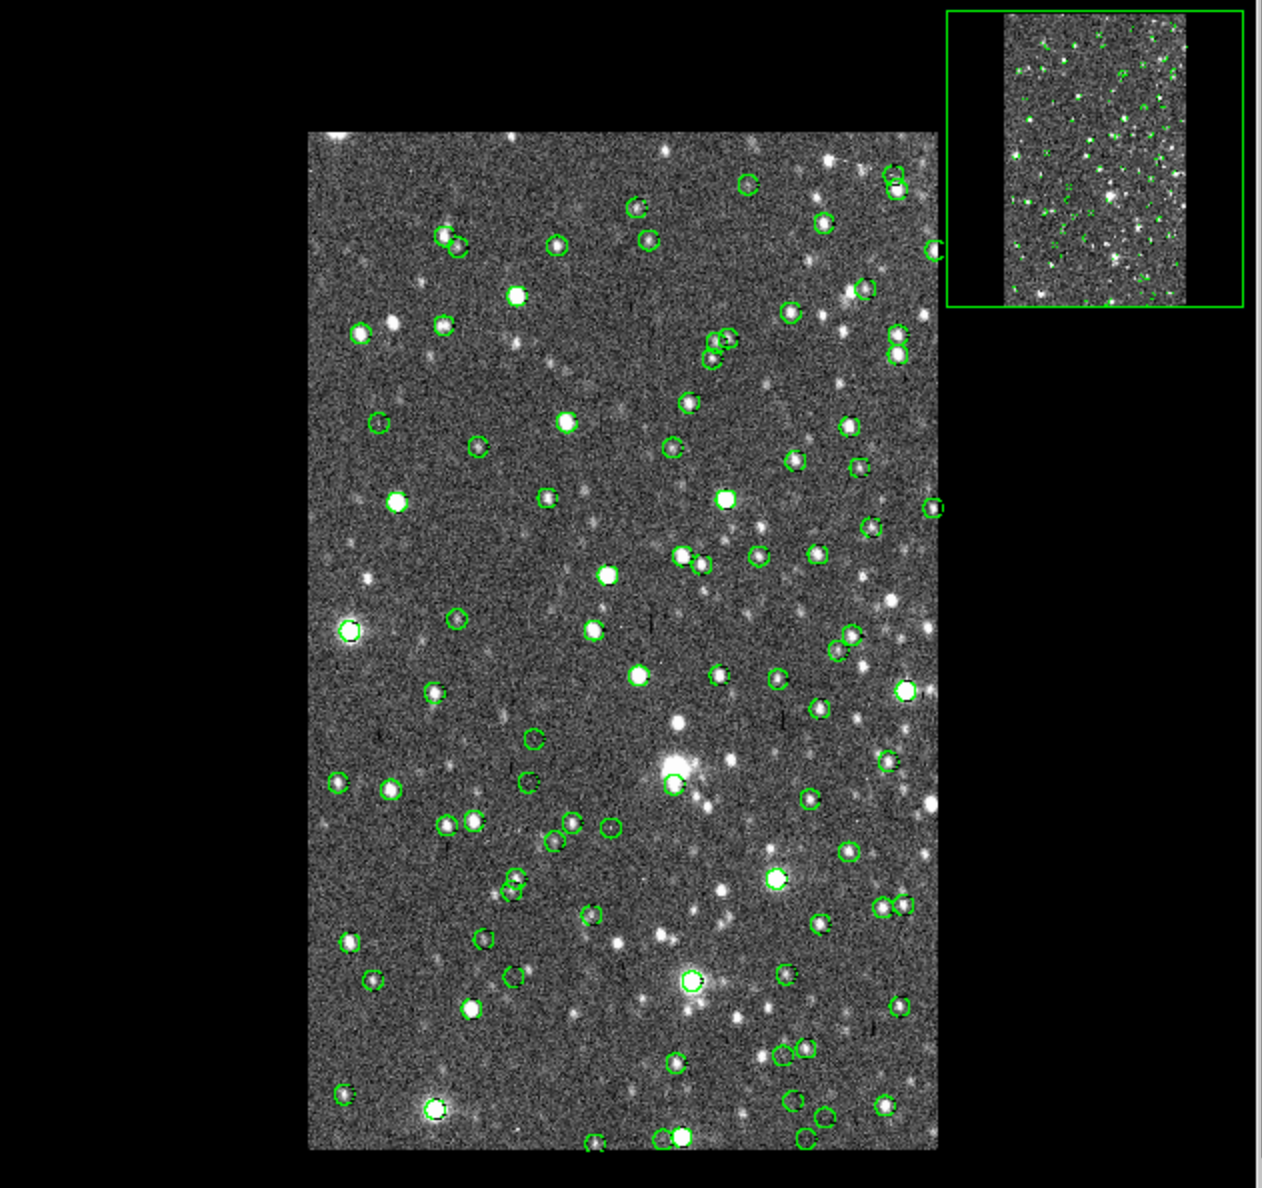
\includegraphics[width=0.6\linewidth]{aceptadas anillo de cielo.png}
    \caption{estrellas aceptadas por el filtro de anillo de cielo}
    \label{fig:placeholder}
\end{figure}

\subsubsection{CMD despues de hacer los procesos de filtrado:}

\begin{figure}[H]
    \centering
    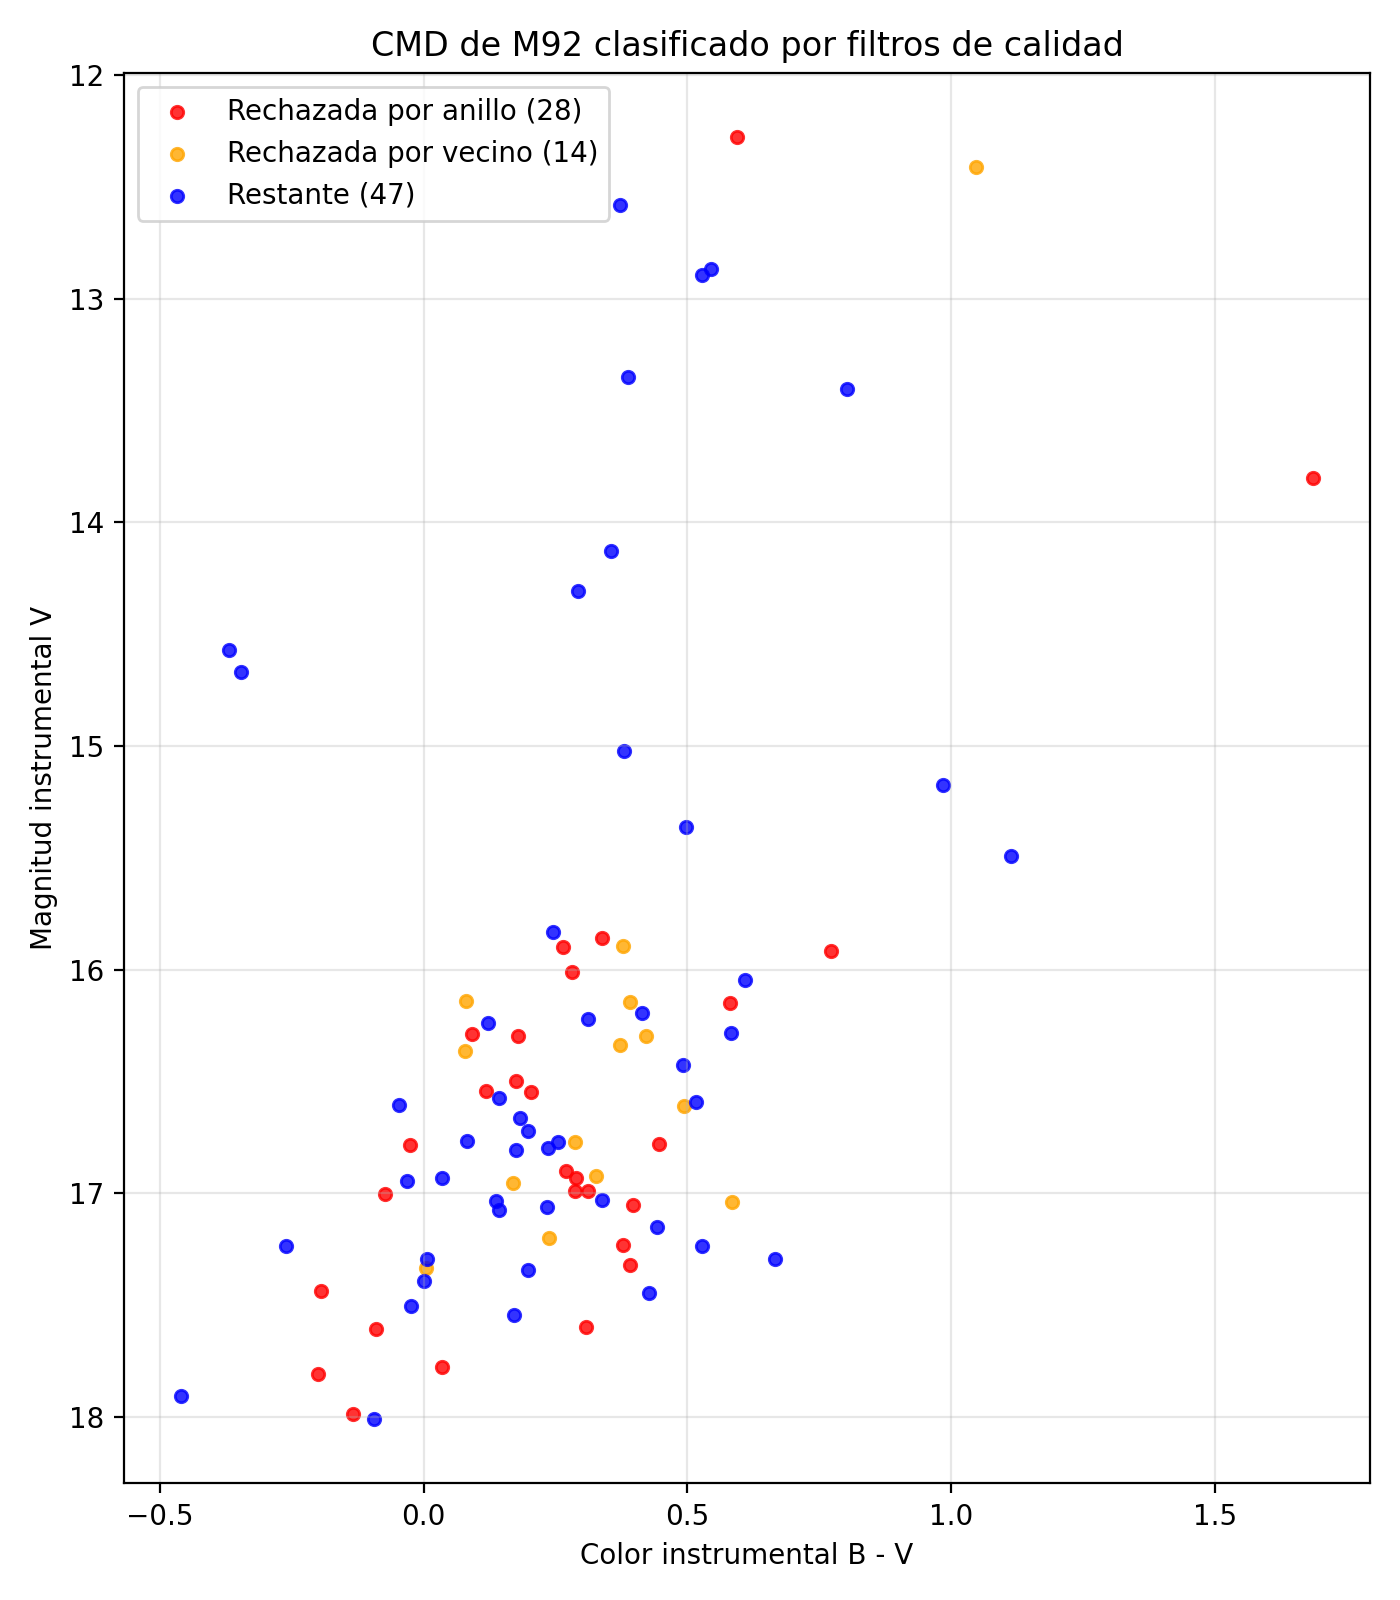
\includegraphics[width=0.5\linewidth]{M92_CMD_coloreado_filtros.png}
    \caption{CMD de la imagen M92011 con las estrellas descartadas por los procesos anteriormente descritos.}
    \label{fig:placeholder}
\end{figure}

% =========================================================
\section{Discusión}
% =========================================================

Los tres talleres permitieron construir un flujo de trabajo progresivo para el análisis de imágenes astronómicas con IRAF. En primer lugar, la reducción CCD fue necesaria para corregir efectos instrumentales presentes en las imágenes crudas. Sin esta etapa, las mediciones posteriores de brillo podrían estar afectadas por el nivel electrónico del detector, regiones no útiles o variaciones de sensibilidad entre píxeles.

El segundo taller permitió entender la importancia de la inspección visual y de las herramientas interactivas. La tarea \texttt{imexamine} fue especialmente útil porque permitió obtener coordenadas, perfiles radiales, estadísticas locales y estimaciones del FWHM. Esta etapa fue importante para aprender a seleccionar estrellas adecuadas, evitando fuentes saturadas, bordes de imagen y estrellas contaminadas por fuentes vecinas.

En el tercer taller se aplicó la fotometría de apertura. La medición del FWHM y del fondo de cielo permitió definir parámetros adecuados para las aperturas y para la detección automática. En el caso de M41, el uso de \texttt{daofind} permitió construir un archivo de coordenadas de estrellas detectadas, mientras que \texttt{tvmark} permitió revisar visualmente si esas detecciones correspondían a fuentes reales.

Las gráficas $MAG$ vs $MERR$ son fundamentales para evaluar la calidad de la fotometría. En general, se espera que las estrellas brillantes presenten errores bajos y que las estrellas débiles tengan errores más altos debido a la disminución de la relación señal-ruido. Si aparecen puntos con errores anormalmente grandes, estos pueden corresponder a estrellas débiles, objetos mal centrados, fuentes contaminadas o detecciones falsas.

% =========================================================
\section{Conclusiones}
% =========================================================

\begin{enumerate}
    \item Se desarrolló un flujo de trabajo en IRAF dividido en tres etapas: reducción CCD, identificación manual de estrellas y fotometría de apertura.

    \item La reducción de las imágenes \texttt{m92010}, \texttt{m92011}, \texttt{m92014} y \texttt{m92015} permitió preparar los datos para realizar mediciones fotométricas más confiables.

    \item El uso de \texttt{display} e \texttt{imexamine} permitió identificar estrellas manualmente, medir posiciones y estimar parámetros importantes como el FWHM y el fondo local.

    \item La fotometría de apertura sobre \texttt{m92011} y M41 permitió obtener magnitudes instrumentales y errores fotométricos.

    \item En el caso de M41, fue necesario separar el archivo multiextensión en canales independientes antes de realizar el análisis.

    \item Las gráficas $MAG$ vs $MERR$ permitieron evaluar la calidad de la fotometría y verificar la tendencia esperada de mayor error en estrellas más débiles.

    \item La metodología desarrollada puede servir como base para una futura calibración fotométrica y para la construcción de diagramas color-magnitud.
\end{enumerate}

% =========================================================
\section{Trabajo futuro}
% =========================================================

Como continuación del trabajo realizado, se propone avanzar hacia la calibración fotométrica de las magnitudes instrumentales. Para ello sería necesario utilizar estrellas estándar, corregir por masa de aire y determinar coeficientes de transformación al sistema fotométrico estándar. Una vez calibradas las magnitudes en diferentes filtros o canales, se podría construir un diagrama color-magnitud y comparar las propiedades observadas con modelos de evolución estelar.

También sería útil comparar los resultados de fotometría de apertura con métodos de fotometría de PSF, especialmente en campos densos donde las estrellas pueden estar muy cercanas entre sí.

% =========================================================
\section{Referencias}
% =========================================================

\begin{thebibliography}{9}

\bibitem{howell2006}
Howell, S. B. (2006). 
\textit{Handbook of CCD Astronomy}. 
Second Edition. Cambridge University Press.

\bibitem{iraf}
Tody, D. (1986). 
The IRAF Data Reduction and Analysis System. 
\textit{Proceedings of SPIE Instrumentation in Astronomy VI}, 627, 733.

\bibitem{massey1997}
Massey, P. (1997). 
\textit{A User's Guide to CCD Reductions with IRAF}. 
National Optical Astronomy Observatories.

\bibitem{davis1989}
Davis, L. E. (1989). 
\textit{A User's Guide to the IRAF Apphot Package}. 
National Optical Astronomy Observatories.

\bibitem{introiraf}
IRAF Tutorial Sessions. 
\textit{Exercise 1: Introduction to IRAF, image display and imexamine}.

\bibitem{photomiraf}
IRAF Tutorial Sessions. 
\textit{Exercise 4: Aperture photometry and photometric calibrations}.

\bibitem{lab5}
Laboratorio 5. 
\textit{Fotometría de apertura de estrellas detectadas en imágenes de M92 en V y B}.

\end{thebibliography}

\end{document}